%%
%% Masterarbeit zum Thema: 
%%

% Definitionen
\def\type{Masterarbeit}
\def\titel{Spezifikationsgesteuerte Abstraktionsverfeinerung f\"ur die formale Verifikation analoger Schaltungen (im Titel lassen sich umlaute nur auf die alte Weise mit slash schreiben)}
\def\author{Name}
\def\matNr{1234567}
\def\abgabedatum{14.\,Mai 2010 }
\def\betreuer{M.\,Sc.\,Julius von Rosen}
\def\pruefI{Prof.~Dr.~L.~Hedrich}
\def\pruefII{Prof.~Dr.~U.~Brinkschulte}


\documentclass[11pt,a4paper,oneside,listsleft,numbers=noenddot]{scrreprt}

% In einstellungen.tex befinden sich alle Einstellungen, die hier oben vorgenommen w�rden. 
% Der gesamte Seitenstil, das Aussehen von lstlistings
%
% Einbindung von n�tigen Pakten
%
\usepackage{makeidx}         % allows index generation
%\usepackage{multicol}        % used for the two-column index
\usepackage[bottom]{footmisc}% places footnotes at page bottom

\usepackage{subfigure}
%\usepackage[bf,hang]{caption2}
\usepackage{algorithm, algorithmic} % F�r Allorithmen
\usepackage{listings}

\usepackage{url}
\newcommand{\urlBiBTeX}[1]{\url{#1}}
%\usepackage{scrpage2}						% Leider keine Ahnung, warum ich das brauche, scheint aber nicht unwichtig zu sein. Kollidiert nur leider mit fancyhdr, wegen chead & cfoot. Daher habe ich es im rahmen der Masterarbeit erstmal auskommentiert
\usepackage[dvips]{color} %pdftex
\usepackage{array}
\usepackage{fancyvrb}

\usepackage{fancyhdr}
\usepackage{german,graphicx,graphics}
%\usepackage{german,fancyhdr,graphicx,graphics}
\usepackage{amsmath,theorem,amsfonts,longtable}
%\usepackage{amsthm}
%\usepackage{enumitem}

% Beschriftung von Bildern, Tabellen, etc
\usepackage{caption3}

%\usepackage{times}
\usepackage{courier}
\usepackage{hyperref}
\usepackage{hhline}
\usepackage[latin1]{inputenc}       %% deutsche Umlaute wie normale Buchstaben verwenden\hyphenation{Sys-tem Sys-tem-mo-dell}


%
% Grundlegende Einstellungen f�r das gesamte Dokument
%
\renewcommand{\baselinestretch}{1.15}\normalsize %Zeilenabstand

\renewcommand{\captionfont}{\small\itshape}
\renewcommand{\captionlabelfont}{\small\normalfont\bfseries}
\renewcommand{\textfraction}{0.05}
\renewcommand{\topfraction}{0.95}
\renewcommand{\bottomfraction}{0.95}
\renewcommand{\floatpagefraction}{0.35}
\setcounter{totalnumber}{5}

\setlength\parskip{\medskipamount}
\setlength\parindent{0pt}

\setlength{\marginparwidth}{1.2cm}  %rechter Rand
\setlength{\textwidth}{15.0cm}    %Textbreite

\setlength{\topmargin}{-1.0cm}    %oberer Rand  -1.0
\setlength{\textheight}{22cm}   %Texth�he
\setlength{\oddsidemargin}{1.2cm} %Linker Rand

% Kleine Ver�nderung von Dictum, damit das so ausschaut, wie ich das haben m�chte
\renewcommand*{\dictumwidth}{.5\textwidth}
\renewcommand*{\raggeddictumtext}{\centering}
%\renewcommand*{\dictumtext}{\setkomafont{}{}}

% Wenn mich nicht alles t�uscht, dann ist der Teil hier f�r die sch�nen Kopfzeilen zust�ndig
\pagestyle{fancy}
\renewcommand{\sectionmark}[1]{\markright{\thesection\ #1}}			%Damit in der Kopfzeile der Section-Name nicht in Uppercase abgebildet wird
\lhead[]{\rightmark}
\rhead[]{} %\thepage
\cfoot{\thepage}
\sloppy
\setlongtables

{\theoremstyle{break}
\newtheorem {beispiel}{Beispiel}[section]
\theoremheaderfont{\scshape\bf}}

\newtheorem {definition}{Definition}[section]
\theorembodyfont{\itshape}
\theoremheaderfont{\scshape\bf}

{\theoremstyle{break}
\newtheorem {satz}{Satz}[section]
\theoremheaderfont{\scshape\bf}}

\setcounter{secnumdepth}{5} 
\setcounter{tocdepth}{3}

%
% Festlegen des Aussehens von lstlistings (Algorithmendarstellungen)
%
\definecolor{hellgrau}{gray}{0.6}				% Definiere Farbe "hellgrau"
\lstloadlanguages{Pascal}
\lstset{%
  numbers=left,										% Position der Nummerierung 
  numberstyle=\normalsize, 
  tabsize=3,
  numbersep=-10pt,               	% Verschiebung der Nummerierung, sodass sie noch im Kasten erscheint
	language=Pascal,								% Sprache ausw�hlen
%	keywordstyle=\bfseries,					% Keywords fett
%	captionpos= bottom,							% Titelposition
	frame=shadowbox,								% Bordertype
	mathescape=true,								% Mathematische Formeln anzeigen
	rulesepcolor=\color{hellgrau},  % Verwende Farbe "hellgrau" als Randfarbe
	showspaces=false,
  showtabs=false,
  columns=fixed,
  breaklines=true
}



\begin{document}
 \pagenumbering{roman}
% \numberwithin{equation}{section}  % Numerierung f�r Gleichungen
% \numberwithin{figure}{section}    % Numerierung f�r Abbildungen
% \numberwithin{table}{section}    	% Numerierung f�r Abbildungen
% \numberwithin{lstlisting}{section}% Numerierung f�r Abbildungen
%\numberwithin{equation}{chapter}  	% Numerierung f�r Gleichungen
% \numberwithin{figure}{section}    % Numerierung f�r Abbildungen
% \numberwithin{table}{section}    	% Numerierung f�r Abbildungen
%\numberwithin{lstlisting}{section} % Numerierung f�r Abbildungen

\begin{titlepage}
  \verb||\\[-2.2cm]
  %\dateCover 

\includegraphics[width=157mm]{picture/EM_Uni_Ffm_Logo6.eps}
\\[4.5cm]
\vspace{0.5cm}
\hrulefill 
\\[0.5cm]
    \vspace{2.0cm}
    \Large \author\rm \\    
    \vspace{1.0cm}
    \LARGE \bfseries \em \begin{center} \titel \end{center} \rm
    \vspace{3.5cm}   
\hrulefill\ \\
\LARGE \type\\
\end{titlepage}
\normalsize

 \newpage                  %
\verb||\\                 % empty page after eides
\vfill
\thispagestyle{empty}


%\def\unilogo{\includegraphics[width=158mm]{picture/EM_Uni_Ffm_Logo.eps}}  %unilogoB.eps
%\newcommand{\dateHeader}
%{ \hbox to 15cm
%  { \parbox[b]{165mm}{\unilogo}
%     \hfill
%  }
%}
\begin{titlepage}
  \verb||\\[-2.2cm]
  %\dateHeader
 
\includegraphics[width=157mm]{picture/EM_Uni_Ffm_Logo6.eps}
  \begin{center}
    \verb||\\
    \vspace{1.4cm}
    \huge \bf \type \rm \\[1mm]
    \Large Institut f�r Informatik\\
    \normalsize Fachbereich Informatik und Mathematik\\
    \vspace{1.5cm}
    \LARGE \bfseries \em 
    \titel \\
    \vspace{1.5cm}
    \large \rm
    \author \\
    Matrikel-Nr.: \matNr \\ \normalsize \vspace{3.0cm}
  \end{center}
    \ \\
    Pr�fer:\\
    \pruefI \\
    \pruefII \\
    \\
    Betreuer:\\
    \betreuer \\
    \\
    Abgabedatum:\\
    \abgabedatum \\
%    \vspace{1.0cm} \\
		\\
%    \vfill
%  \begin{center}
    \rm \normalsize Frankfurt am Main, \today
%  \end{center}
\end{titlepage}
%\thispagestyle{empty}
\normalsize


\thispagestyle{empty}
\vspace*{2cm}
\section*{Danksagung}

Hier k�nnte Ihre Werbung stehen!
(A tribute to JD )


    
\verb||\\                 %
\vfill                    % empty page after the title page
\thispagestyle{empty}     %

\newpage

\verb||\\
\vfill
\begin{quote}
\thispagestyle{empty}
\vfill{
{\flushleft \textbf{Eidesstattliche Versicherung}}
\\*[0.5cm]
Hiermit versichere ich, dass ich die vorliegende Arbeit
selbstst�ndig und nur unter Verwendung der angegebenen
Hilfsmittel angefertigt habe.
\\*[0.1cm]

{\flushleft Frankfurt am Main, \today}\\*[0.5cm]}

{\flushleft \author}
\end{quote}

\newpage                  %
%\verb||\\                 % empty page after eides
%\vfill
%\thispagestyle{empty}
  % Eidesstattliche Versicherung
%   \newpage
\thispagestyle{empty}
\chapter*{Aufgabenstellung}
\thispagestyle{empty}

Verfahren zum Model-Checking analoger Schaltungen basieren auf einer vollst�ndigen Diskretisierung des Zustandsraums. Diese Diskretisierung �berf�hrt den kontinuierlichen Zustandsraum in eine Graph-Datenstruktur, auf der temporallogische Model Checking - Algorithmen angewendet werden k�nnen. Diese vollst�ndige Diskretisierung des Zustandsraums vor Anwendung der Verifikationsalgorithmen ist sehr rechenzeitintensiv und abh�ngig von der auszuwertenden Spezifikation wird nur ein kleiner Teil des erzeugten Modells untersucht. 

Dementsprechend ist das Ziel dieser Arbeit, eine Methodik zu entwickeln, die abh�ngig von der zu klassifizierenden Spezifikation eine Verifikation nur auf den relevanten Teilen des Zustandsraums durchf�hrt. Dies soll auf Basis einer Abstraktionsverfeinerung durch schrittweise Exploration des Zustandsraums erfolgen, womit eine on-demand Diskretisierung der relevanten Zustandsraumgebiete durch transiente Simulationstrajektorien erreicht wird.

Als Arbeitsumgebung wird eine Schnittstelle zu einem Simulationswerkzeug f�r analoge
Schaltungen f�r die Abtastung des Zustandsraums sowie eine auf GNU Octave basierende
Entwicklungsumgebung zur Verf�gung gestellt.


%   \newpage

 
\tableofcontents
    \newpage 
\addcontentsline{toc}{section}{Abk�rzungsverzeichnis}
 %\thispagestyle{empty}
%\textbf{\Large{Abk�rzungsverzeichnis}}
%\\[1.0cm]

\chapter*{Abk�rzungsverzeichnis}

\begin{tabular}{p{0.18\textwidth}  p{0.8\textwidth}}
%\textbf{EDA} \dotfill{} &\emph{Electronic Design Automation}\\ % \newline (dt. Hardwarebeschreibungssprache)
%\textbf{VHDL} \dotfill{} &\emph{Very High Speed Integrated Circuit Hardware Description Language}\\ % \newline (dt. Hardwarebeschreibungssprache)
\textbf{AABB} \dotfill{} &\emph{Axis-Aligned Bounding Box}\\
\textbf{DEA} \dotfill{} &\emph{Deterministischer endlicher Automat}\\
\textbf{NEA} \dotfill{} &\emph{Nichtdeterministischer endlicher Automat}\\
\\
\textbf{LTL} \dotfill{} &\emph{Linear Temporal Logic}\\
\textbf{CTL (-AT)} \dotfill{} &\emph{Computation Tree Logic (- Analog Timed)}\\
%\textbf{MTL} \dotfill{} &\emph{Metric Temporal Logic}\\
\textbf{ASL} \dotfill{} &\emph{Analog Specification Language}\\
\\
%\textbf{DAE} \dotfill{} &\emph{Differential Algebraic Equation \newline (dt. Algebro-Differentialgleichung)}\\
\textbf{DAE} \dotfill{} &\emph{Differential Algebraic Equation (dt. Algebro-Differentialgleichung)}\\
%\textbf{MNA} \dotfill{} &\emph{Modified Nodal Analysis (dt. Modifizierte Knoten-Analyse)}\\
\textbf{CMRR} \dotfill{} &\emph{Common Mode Rejection Ratio (dt. Gleichtaktunterdr�ckungsverh�ltnis)}\\
\textbf{PSRR} \dotfill{} &\emph{Power Supply Rejection Ratio \newline (dt. Netzst�rungsunterdr�ckungsverh�ltnis)}\\
\textbf{SR} \dotfill{} &\emph{Slew Rate (dt. Flankensteilheit)}\\
\textbf{VCO} \dotfill{} &\emph{Voltage-Controlled Oscillator (dt. Spannungsgesteuerter Oszillator)}\\
\\
\textbf{OG} \dotfill{} &\emph{Obergrenze eines Intervalls}\\
\textbf{UG} \dotfill{} &\emph{Untergrenze eines Intervalls}\\
\end{tabular}

\newpage

    \newpage
\addcontentsline{toc}{section}{Formelzeichen}
 %\thispagestyle{empty}

%\textbf{\Large{Formelzeichen}}
%\\[1.0cm]

% \addcontentsline{toc}{section}{Abk�rzungsverzeichnis}

\chapter*{Formelverzeichnis}
%\section*{Formeln}

%\begin{tabular}{p{4cm}  l}
\begin{tabular}{p{0.25\textwidth}  p{0.7\textwidth}}
\textbf{$\mathbb N$} \dotfill{} & Menge der nat�rlichen Zahlen\\ 
\textbf{$\mathbb R$} \dotfill{} & Menge der reellen Zahlen\\ 
\textbf{$\mathbb Q$} \dotfill{} & Menge der rationalen Zahlen\\ 
\\
\textbf{$\vec x$} \dotfill{} & Skalar oder Vektor\\ 
\textbf{$\vec x_i$} \dotfill{} & $i$-te Komponente des Vektors $x$\\ 
\textbf{$t$} \dotfill{} & Zeit\\ 
\textbf{$\left[UG,OG\right]$} \dotfill{} & Intervall mit Untergrenze $UG$ und Obergrenze $OG$\\ 
\textbf{$\tau$} \dotfill{} & �berschneidungsgrad zweier Bounding Boxen (in \%)\\ 
\textbf{$dim$} \dotfill{} & Dimension des Zustandsraums \\ 
\textbf{$sw_i$} \dotfill{} & Schrittweite der Transition${}_i$ \\ 
\textbf{$sw_j ^{OG}$} \dotfill{} & Schrittweitenobergrenze der Punktmengentransition${}_j$ \newline (durchschnittliche Schrittweite der Transitionen der Punktmenge) \\ 
\\
\textbf{$f(x)$} \dotfill{} & Skalar- oder vektorwertige Funktion in Abh�ngigkeit von $x$\\ 
\textbf{$\dot x(t) = \frac{dx}{dt} $} \dotfill{} & Erste Ableitung des Vektors $x$\\ 
\textbf{$f \bigl( \dot x(t), x(t), t \bigr) = 0$} \dotfill{} & Algebro-Differentialgleichungssystem \\ 
\\
%\textbf{A} \dotfill{} & Matrix\\ 
\textbf{$\mathcal A$} \dotfill{} & Menge\\ 
\textbf{$A$} \dotfill{} & Operator einer temporalen Logik\\ 
\textbf{$\Phi$} \dotfill{} & Ausdruck in temporaler Logik\\ 
\\
\textbf{$KS$} \dotfill{} & Zustandsgraph in Kripke-Struktur\\ 
\\
%$f_s$ \dotfill{} &Abtastfrequenz\\
%$\triangle f$ \dotfill{} &Spektrallinienabstand\\
%$t_{\lambda}$ \dotfill{} &Zeitdauer eines Zeitfensters\\
%$\alpha$ \dotfill{} &konstanter Gl{\"a}ttungsfaktor\\
%$\alpha (\lambda,k)$ \dotfill{} &zeit- und frequenzabh{\"a}ngiger Gl{\"a}ttungsfaktor\\
%$\alpha_c(\lambda)$ \dotfill{} &Korrektur des Gl{\"a}ttungsfaktors\\
%$\alpha_{max}$ \dotfill{} &maximaler Gl{\"a}ttungsfaktor\\
%$\alpha_{min}$ \dotfill{} &minimaler Gl{\"a}ttungsfaktor\\
%$\alpha_{opt}(\lambda,k)$ \dotfill{} &optimaler Gl{\"a}ttungsfaktor\\

%$\beta(\lambda,k)$ \dotfill{} &Gl{\"a}ttungsfaktor f{\"u}r die
%                               Momente erster und zweiter Ordnung\\
%$\epsilon$ \dotfill{} &\emph{subfloor} Konstante\\
%$\gamma$ \dotfill{} &\emph{oversubstraction factor}\\
%$\overline{\gamma}$ \dotfill{} &\emph{a posteriori SNR}\\
%$\Gamma(\cdot)$ \dotfill{} &Gammafunktion\\
%$k$ \dotfill{} &Frequenzindex\\
%$\lambda$ \dotfill{} &Zeitindex\\
%$\Omega_k$ \dotfill{} &Mittenfrequenz\\
%$\sigma^2_n$ \dotfill{} &Varianz des St{\"o}rger{\"a}usches n\\
%$\sigma^2_s$ \dotfill{} &Varianz des Sprachsignals s\\
%$\vartheta$ \dotfill{} &Vergleichsoperationen pro
%                        Zeitschritt und Frequenz\\
%$\varrho$ \dotfill{} &Steigung des Rauschleistung\\
%$\delta$ \dotfill{} &maximale Zeitverz{\"o}gerung\\
%$\chi$ \dotfill{} & Durchschnitt aller gemessenen Peakbreiten\\
%                  & f{\"u}r alle Frequenzen\\
%$\varphi_{xs}$ \dotfill{} & Kreuzkorrelationen der Signale x und s\\
%$\phi_{xx}$, $\phi_{ss}$, $\phi_{nn}$ \dotfill{}
%       &Autokorrelationen der Signale x, s, n\\
%$\Theta$ \dotfill{}
%                &Leistungsdichtespektrum\\[0.5cm]
\end{tabular}


    \newpage


\pagenumbering{arabic}

\chapter{Einleitung \label{ch_einleitung}}

Seit fast einem halben Jahrhundert existiert das von Gordon Moore formulierte Gesetz, dass sich die Transistoranzahl auf einem Chip innerhalb von zwei Jahren verdoppelt. 
Dieser rapide wachsenden Schaltungskomplexit�t versuchen seit jeher Industrie und Forschung mit verbesserten Entwurfsprozessen zu begegnen. Gerade der in der Industrie vorherrschende Innovationsdruck f�r neue Produkte und die immer k�rzer werdende Lebensdauer eben dieser, fordern einen Schulterschluss. Doch in der Realit�t existiert ein sogenannter, stetig wachsender \glq Design Gap\grq{} zwischen der Schaltungskomplexit�t und dem Entwurfsprozess. 
%sieht anders aus und wird im sogenannten  dargestellt. %Der \glq Design Gap\grq{} zeigt den Unterschied der theoretisch fertigbaren und der praktisch entwerfbaren Schaltungen. ODER
Abstrakt formuliert, zeigt der \glq Design Gap\grq{} den Unterschied der theoretisch fertigbaren und der praktisch entwerfbaren Schaltungen.

...


\section*{Aufbau dieser Arbeit} 

Diese Arbeit betrachtet ... 


 \newpage

\chapter{Grundlagen \label{ch_grund}}

Dieses Kapitel beschreibt die Grundlagen, ...


\section{Von der Spezifikation zur Verifikation \label{sec:spezi}}

Bei der Herstellung von analogen, digitalen oder mixed-signal Schaltungen wird von der Idee bis zur Fertigstellung ein definierter Prozess durchlaufen. Dieser beinhaltet folgende Schritte:
\begin{enumerate}
	\item die Spezifikation \label{proz_spez}
	\item den Entwurf
	\item die Fertigung
	\item den Test
\end{enumerate}


...

Grammatik \eqref{eq:CTL-AT} repr�sentiert die Erweiterung der CTL - Syntax um die Neuerungen von CTL-A und CTL-AT.
\begin{align}
	\label{eq:CTL-AT}
	\Phi  \ :=  \ a  \ & | \ z \: \ast \: v \ | \ \Phi \: \circ \: \Psi \ | \ \neg \: \Phi \   \\
	& | \ \triangleright \: \diamond \: \Phi \ | \ \triangleright \: \Phi \: U \: \Psi \ | \ \triangleright \: \diamond^{-1} \: \Phi \ | \ \triangleright \: \Phi \: U^{-1} \: \Psi	 \notag \\
	& | \ \triangleright \: \diamond \: \Box \: \Phi \ | \ \triangleright \: \Phi \: U \: \Box \: \Psi \ | \ \triangleright \: \diamond^{-1} \: \Box \: \Phi \ | \ \triangleright \: \Phi \: U^{-1} \: \Box \: \Psi \notag
\end{align}
Zieht man \cite{HartongKlaHed04} f�r die Beschreibung der CTL-AT - Syntax die Grundlage der CTL-Syntax auf Tabelle \ref{tab:ctlat} , die Erweiterung aus Tabelle \ref{tab:ctlat} auf Seite \pageref{tab:ctlat}und die neu formulierten Zeitbedingungen hinzu, erh�lt man Tabelle \ref{tab:ctlat}. Die neuen Variablen und die analogen Operatoren reihen sich direkt nach der bool'schen Zustandsvariablen ein. Abgeschlossen wird die Syntaxbeschreibung nun von dem Vergangenheitsoperator und den Zeitbedingungen.
Diese werden an die temporalen Operatoren, mit Ausnahme des $X$-Operators, als Zeitintervall angeh�ngt, sodass eine minimale und maximale zeitliche Pfadl�nge definiert ist. Eine Operatorenschreibweise $\triangleright \ X \ \Box \: \Phi $ bzw. $ \triangleright \ X^{-1} \ \Box \: \Phi $ ist nicht zul�ssig.
\begin{table}[htb]
\centering
\caption[Beschreibung der CTL-AT - Syntax]{Beschreibung der CTL-AT - Syntax (Quelle: \cite[S. 10]{platte})}
\begin{tabular}{|p{0.02\textwidth}|p{0.37\textwidth}|p{0.4\textwidth}|}
\hline
$a$ & Bool'sche Zustandsvariable &  \\ \hline
$z$ & Kontinuierliche Zustandsvariable &  \\ \hline
$v$ & Reeller Zahlenwert ($ \mathbb{R} $) &  \\ \hline
\multicolumn{ 1}{|l|}{$\ast$} & \multicolumn{ 1}{l|}{Analoge Operatoren} & $\ > \ = \ $ gr��er \\ \cline{ 3- 3}
\multicolumn{ 1}{|l|}{} & \multicolumn{ 1}{l|}{} & $\ < \ = \ $ kleiner \\ \hline
\multicolumn{ 1}{|l|}{$\circ$} & \multicolumn{ 1}{l|}{Bool'sche Operatoren} & $\ \vee \ = \ $ oder \\ \cline{ 3- 3}
\multicolumn{ 1}{|l|}{} & \multicolumn{ 1}{l|}{} & $\ \wedge \ = \ $ und \\ \cline{ 1- 1}\cline{ 3- 3}
$\neg$ & \multicolumn{ 1}{l|}{} & $\ \neg \ = \ $ nicht \\ \hline
\multicolumn{ 1}{|l|}{$\triangleright$} & \multicolumn{ 1}{l|}{Pfadquantoren} & $\ A \ = \ $ auf allen Pfaden \\ \cline{ 3- 3}
\multicolumn{ 1}{|l|}{} & \multicolumn{ 1}{l|}{} &  $\ E \ = \ $ auf mindestens einem Pfad \\ \hline
\multicolumn{ 1}{|l|}{$\diamond$} & \multicolumn{ 1}{l|}{Temporale Operatoren} & $\ X \: = \ $ n�chster Zeitschritt (neXt) \\ \cline{ 3- 3}
\multicolumn{ 1}{|l|}{} & \multicolumn{ 1}{l|}{} & $\ F \ = \ $ irgendwann (Finally) \\ \cline{ 3- 3}
\multicolumn{ 1}{|l|}{} & \multicolumn{ 1}{l|}{} & $\ G \ = \ $ immer (Globally) \\ \cline{ 1- 1}\cline{ 3- 3}
$U$ & \multicolumn{ 1}{l|}{} & $\ U \ = \ $ bis (Until) \\ \hline
\multicolumn{1}{|r|}{${}^{-1}$} & Vergangenheit & $ $ Umkehrung der Zeit \\ \hline
$\Box$ & Zeitintervall & $\ \left[ t_{low}, t_{high} \right] $ mit: \newline $ \ t_{low} \in {\mathbb R}^{+} _{0}, \ t_{high} \in {\mathbb R}^{+} \ $ \newline $  t_{low}\ \leq \ t_{high}$ \\ \hline
\end{tabular}
\label{tab:ctlat}
\end{table}


...

 \newpage

%\chapter{Die Operationen \label{ch:funk}}

...

\section{Die Operatoren $E$ und $U$ \label{sec:eu} }
%\section{Die $E \: \Phi \: U \: \Psi $ - Operation \label{sss:eu} }
\subsubsection*{Die $E \: \Phi \: U \: \Psi $ - Operation \label{sss:eu} }

Die Operationen dienen dem Model-Checking als eine Pr�finstanz der Eigenschaften und der Spezifikation. Dazu werden der Schaltung mittels der Operatoren sinnbildlich Fragen gestellt, deren Antworten die Richtigkeit einer Eigenschaft/Bedingung widergeben. 
Die f�r die $E \: \Phi \: U \: \Psi $ - Operation formulierte Frage w�rde wie folgt aussehen:
%(Ab�ndern)In Worten l�sst sich die $E \: \Phi \: U \: \Psi $ - Operation wie folgt ausgedr�ckt:
\begin{description}
  \item[] Auf welchen Pfaden gilt $\Phi$, bis unmittelbar danach $\Psi$ gilt?
\end{description}
%Es gilt immer $\Psi$ bis $\Phi$ gilt. Es existiert kein Pfad, auf dem $\neg\Phi$ gilt bis $\neg\Psi$ und $\neg\Phi$ gelten und es existiert kein Pfad, auf dem $\Phi$ nie g�ltig wird.
Im \textbf{zeitunbeschr�nkten} Fall, werden durch $E \: \Phi \: U \: \Psi $ die Zust�nde in die Ergebnismenge eingef�gt, die auf einem Pfad in $\Phi$ liegen, welcher unmittelbar nach $\Phi$ in $\Psi$ landet. F�r die gefundenen Zust�nde gilt somit, dass auf mindestens einem Pfad $\Psi$ unmittelbar auf $\Phi$ folgt.
Eine \textbf{Zeitbeschr�nkung} erschwert die Erf�llbarkeit von $E \: \Phi \: U \: \Psi $. Der Operator $E \: \Phi \: U \left[ t_{low}, t_{high} \right] \: \Psi $ restriktiert die Erf�llung auf ein Zeitintervall. Nur Zust�nde von Pfaden, die innerhalb von $\left[ t_{low}, t_{high} \right]$ von $\Phi$ unmittelbar nach $\Psi$ kommen, werden zur Ergebnismenge hinzugef�gt.
Daraus l�sst sich ableiten, dass folgende Teilmengenrelation zu gelten hat: 
\begin{equation}
  E \: \Phi \: U \left[ t_{low}, t_{high} \right] \: \Psi \ \subseteq  E \: \Phi \: U \: \Psi .	\notag
\end{equation}
Abbildung \ref{fig:eu_z} zeigt einen Zustandsgraphen und die jeweilige Ergebnismenge, die aus der Fallunterscheidung \glq keine und eine zeitlichen Begrenzung\grq{} resultiert. Die gr�n markierten Knoten stellen die Zust�nde dar, die in der Ergebnismenge enthalten sind. Des Weiteren zeigen die gr�nen Kanten die Pfade an, anhand denen die Ergebnismenge zur Erf�llung der CTL-AT - Operationen bestimmt wurde.
Diese Angaben gelten f�r das restliche Kapitel.
\begin{figure}[htb]
  \centering
  \begin{minipage}[b]{7 cm}
   \subfigure[ ]
   {
    \includegraphics[width=\textwidth]{picture/Graphen/eu_zub.eps}
    \label{fig:eu_zub}  
    }
  \end{minipage}
  \begin{minipage}[b]{7 cm}
   \subfigure[ ]
   {
    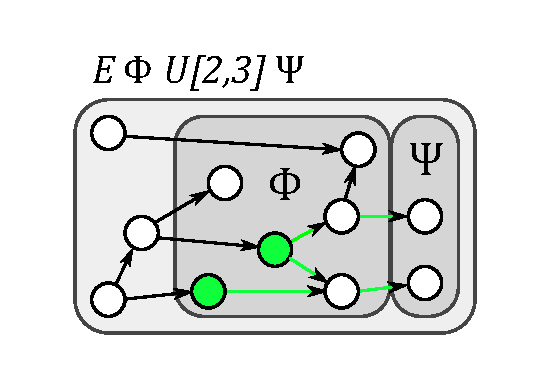
\includegraphics[width=\textwidth]{picture/Graphen/eu_zb.eps}
    \label{fig:eu_zb}
    }
  \end{minipage}
  \caption[Zustandsgraph mit Ergebnismenge einer $E \: \Phi \: U \: \Psi $ - Operation]{Beispielhafter Zustandsgraph f�r die  $E \: \Phi \: U \: \Psi $ - Operation mit Fallunterscheidung in Zeitunbeschr�nkung \ref{fig:eu_zub} und Zeitbeschr�nkung \ref{fig:eu_zb} }
  \label{fig:eu_z}
\end{figure}


...

% \newpage
%\chapter{Zustandsraumexploration \label{ch_zustand}}

Die Erforschung des Zustandsraumes analoger Schaltungen f�r die Verifikation ist mit erheblichen Schwierigkeiten verbunden.
% und harrt der L�sungen. 
%stellt sich weiterhin als ein schwieriges Terrain heraus. 
Allgemein betrachtet, ist der Zustandsraum eine formale Abbildung des Verhaltens der Schaltung. F�r die digital-technische Verifikation entspricht der Zustandsraum einem Quadrupel (die Gesamtmenge an Zust�nden, die Zustands�bergangsrelationen, eine nicht-leere Menge an Startzust�nden und eine nicht-leere Menge an Zielzust�nden), der als Automat das Systemverhalten zeigt. F�r analoge Schaltungen l�sst sich das Systemverhalten nicht mehr als eine diskrete Menge an Zust�nden abbilden. Vielmehr wird die wertkontinuierliche Zustandsmenge von einem mehrdimensionalen Differentialgleichungssystem aufgespannt. Die Dimensionsgr��e wird von der Anzahl der Variablen und der Anzahl der energiespeichernden Komponenten bestimmt und bewirkt, dass die Gr��e des Zustandsraumes exponentiell w�chst. 

Des Weiteren k�nnen in nicht-deterministischen Automaten pro Zustand mehrere Nachfolger existieren, sodass die zu pr�fende Zustandsmenge um ein Vielfaches anw�chst. Dieses Wachstum, auch \glqq Zustandsraumexplosion\grqq{} genannt, ist unter dem Begriff \glq Model-Checking Problem\grq{} in der Forschung bekannt\cite{Clarke03ce-ga}. 
Es erkl�rt auch, warum der bisherige Forschungsansatz \glqq die vollst�ndige Diskretisierung\grqq{} eine $np$-harte Komplexit�tsklasse nach sich zieht und damit f�r gen�gend gro�e Schaltungen unbrauchbar wird.
Jedoch ist dies nicht die einzige Herausforderung, der sich das Model-Checking analoger Schaltungen stellt. Es existieren weitere Schranken f�r die Diskretisierung von analogen Schaltungen, die die Komplexit�t der Verifikation erh�hen. 
Die Berechnung des Zustandsraums fordert ein hohes Ma� an Rechenleistung. Dies basiert zum einen auf der Abbildung des analogen Schaltungsverhaltens auf ein diskretes Transitionssystem und zum anderen auf der Durchf�hrung der formalen Verifikation zur Pr�fung der Bedingungen. Mit der Erh�hung des Grades der Genauigkeit der Abbildung und/oder der Verifikation steigt die geforderte Rechenleistung exponentiell. %Die Anzahl der Zust�nde eines modellierten analogen Systems w�chst exponential mit der Anzahl an Variablen und Energie-speichernden Komponenten.
Auch der Visualisierung der Ergebnismengen ist eine Grenze durch das r�umliche Vorstellungsverm�gen des Menschen gesetzt. Eine Visualisierung muss daher auf drei Dimensionen begrenzt werden, um Designern nach dem Model-Checking die Chance zu geben, mit der Ergebnismenge arbeiten zu k�nnen. Ausnahmen mit Darstellungen von vier Dimensionen existieren jedoch \cite{peterDA}. 
%Mehr als drei Dimensionen kann sich der Mensch praktisch nicht vorstellen.

%HMMM: Model-Checking an sich ist effizient, wird aber durch den hohen Speicherplatzbedarf ausgebremst. 
Zusammenfassend sind die drei entscheidenden Schranken, in denen sich die Verifikation von analogen Schaltungen bewegt, 
\begin{itemize}
	\item die Darstellung des Zustandsraums analoger Schaltungen,
	\item die Diskretisierung des analogen Zustandsraumes und
	\item die M�glichkeit der Visualisierung der Ergebnisse.
\end{itemize}

Die drei Schranken werden in den folgenden drei Abschnitten \ref{sec:zustandsraum} bis \ref{sec:visuZust} analysiert und daraus resultierend L�sungen zur Problemreduktion erarbeitet.


\section{Zustandsraum-Darstellung analoger Schaltungen \label{sec:zustandsraum}}

Eine analoge Schaltung l�sst sich anhand eines nichtlinearer Algebro-Differentialgleichungssystems erster Ordnung (engl. nonlinear first order differential algebraic equation) formal beschreiben \cite{har03mod,steinhorst09joint}. Die Algebro-Differentialgleichungen (DAE) setzen sich dabei aus expliziten gew�hnlichen Differentialgleichungen, gekoppelt mit algebraischen Nebenbedingungen, zusammen. Die Nebenbedingungen sind ableitungsfrei. 

F�r die systembeschreibenden DAE einer analogen Schaltung m�ssen folgende drei Parameter definiert werden:
\begin{enumerate}
	\item Input-Vektor $u(t)$ (Eingangsvariablen)
	\item Vektor mit den Systemvariablen $x(t)$
	\item Vektor, mit der ersten Ableitung der Systemvariablen $\dot x(t)$
\end{enumerate}
Formel \eqref{eq:as_dae} zeigt die Differentialgleichung zur Darstellung analoger Systeme: %, die zu gelten hat.
\begin{equation}
	f \bigl( \dot x(t), x(t), u(t) \bigr) = 0
	\label{eq:as_dae}
\end{equation}
Die beiden Vektoren $u(t)$ und $x(t)$ werden durch eine erweiterte \glqq modifizierte Knotenanalyse\grqq{}(engl. Modified Nodal Analysis (MNA)), die auf die Netzliste der Schaltung angewandt wird, gewonnen. 
%http://www.analog-electronics.eu/analog-electronics/modified-nodal-analysis/modified-nodal-analysis.xhtml
% Hier ist eine gute Beschreibung geliefert => ggf f�r eine Quellen-Angabe
Der Zustandsraum aus dem daraus resultierenden Algebro-Differentialgleichungssystem wird von den Input-Variablen und den energiespeichernden Systemvariablen $x_e(t)$, wie beispielsweise Kapazit�ten oder Induktivit�ten, aufgespannt.
Anschlie�end werden im aufgespannten Raum Zufalls-Messpunkte gleichm��ig verteilt. Daraus werden, basierend auf numerischen Integrationsschritten mit einer kurzen, konstanten Integrationszeit, die das Verhalten der Ableitung der Systemvariablen $\dot x_e(t)$ repr�sentiert, weitere Messpunkte generiert. 
Durch die Schrittweitensteuerung steigt die Dichte der Messpunkte in den Gebieten von nicht-homogenem Systemverhalten. 
So ergibt sich ein diskretes Vektorfeld $V_D$ mit einer Menge an Messpunkten $Q = \left\{ q_1, \: \ldots, \: q_m \right\} $, das eine Schaltung modelliert.
Es wird also ein Vektorfeld $V : \mathbb R^n \ \rightarrow \ \mathbb {R}^n $ mit einer diskreten Menge $Q = \left\{ q_1, \: \ldots, \: q_m \right\}$ mit $m$ Messpunkten $q_i$ betrachtet. F�r diese diskrete Menge gilt, dass im Zustandsraum das diskrete Vektorfeld $V_D : Q \ \rightarrow \ V_D $ als 
\begin{equation}
	V_D (q_i) = \left\{ v_i \; | \; \exists q_i \in Q : v_i = \frac{\delta q_i}{\delta t} \right\} \notag
\end{equation}
definiert ist.
Das diskrete Vektorfeld $V_D$ wird demnach von den Ortsvektoren $p_i$ abgebildet, welche neben den Messpunkten auch die Richtungsvektoren $v_i = V_D(q_i)$ mit ihrer Bewegungsrichtung und Geschwindigkeit ausweisen.
%Der Sampling-Prozess wird gef�hrt von der Divergenz der L�nge und Winkel von benachbarten Vektoren.
Diese Modellierung des Vektorfeldes wird von dem prototypischen Werkzeug \textit{amcheck}\footnote{\textit{amcheck} ist ein Model-Checker f�r analoge Schaltungen mit Zeitbedingungen. Er wurde am Institut f�r Mikroelektronische Schaltungen der Universit�t Hannover entwickelt. \cite{har03mod} } 
genutzt. 
%(Wir betrachten ein Vektorfeld $V : \mathbb R^n \ \rightarrow \ \mathbb {R}^n $ in welchem f�r die diskrete Menge $Q = \left\{ q_1, \: \ldots, \: q_m \right\}$ mit $m$ Sampling-Punkten $q_i$ im Zustandsraum das diskrete Vektorfeld $V_D : Q \ \rightarrow \ V_D $ als 
%\begin{equation}
%	V_D (q_i) = \left\{ v_i \; | \; \exists q_i \in Q : v_i = \frac{\delta q_i}{\delta t} \right\}
%\end{equation}
%definiert ist. )
%We consider a vector field V : Rn ! Rn on which for the discrete set Q = {q1, ..., qm} of m sample points qi in the state space the discrete vector field VD : Q ! VD is defined:
%(Das diskrete Vektorfeld $V_D$ wird von den Positionsvektoren $p_i$, welche die Sampling-Punkte im Zustandsraum und die Bewegungsrichtung der Richtungsvektoren $v_i = V_D(q_i)$ ermitteln, inklusive der Geschwindigkeit innerhalb $V$ an Position $q_i$, repr�sentiert.)
%In other words, the discrete vector field VD is represented by position vectors qi determining the sample points in the state space and the direction vectors vi = VD(qi) giving the motion direction and speed within V at position qi.
Eine genauere Beschreibung der Modellierung des Zustandsraumes anhand einer DAE ist in \cite{steinhorst09state} zu finden.
%, inklusive Beispiele an Schaltungen,
%

\section{Vollst�ndige Diskretisierung analoger Schaltungen \label{sec:stand}}

Der aktuelle Stand der Technik basiert auf den Algorithmen und Techniken der formalen Verifikation, die f�r digitale Schaltungen entwickelt wurden.
%Das Model-Checking ist da keine Ausnahme. 
Es exisitieren kommerzielle Softwarel�sungen, die Aussagen �ber die Funktionalit�t, das Timing-Verhalten und andere spezifizierte Kriterien treffen. Daher sind sie in den Entwurfsprozess der Chipentwicklung von digitalen Schaltungen integriert.

Die formale Verifikation von analogen Schaltungen befindet sich im Gegensatz dazu im Anfangsstadium der Entwicklung. Das prototypische Werkzeug \textit{amcheck} wurde im Rahmen von \cite{platte} von CTL-A auf CTL-AT % erweitert. 
f�r einen geeigneten Einsatz im Model-Checking analoger Schaltungen erweitert. 
Neben der Erreichbarkeits- und der Fixpunktanalyse lassen sich zeitliche Kriterien, wie Verz�gerungszeiten, pr�fen. Jedoch gilt f�r \textit{amcheck}, wie f�r alle bisherigen Verfahren, dass sie das Verhalten einer analogen Schaltung diskretisieren. Erst auf dem diskretisierten Zustandsraum werden die Pr�fungen der Spezifikation bzw. des Systemverhaltens durchgef�hrt. 

\subsection{Stand der Technik \label{ss:vollDis}}

Die vollst�ndige Diskretisierung nach \cite{har03mod}, die momentan f�r das Model-Checking analoger Schaltungen durchgef�hrt wird, ist ein erheblicher Mehraufwand gegen�ber dem Model-Checking digitaler Schaltungen.
%Das Systemverhalten wird dabei so wenig wie m�glich ver�ndert.
Die Diskretisierung des kontinuierlichen, unendlichen Zustandsraums beginnt mit der Begrenzung desselben durch Festlegen der Intervallgrenzen der Zustandsvariablen. 
Die Begrenzung wird anhand einiger vorliegender Angaben der Spezifikation, wie zum Beispiel die Betriebs-, Eingangs- oder Ausgangsspannung, bestimmt und der Zustandsraum auf den zu betrachtenden Bereich reduziert. 
Als Zweites folgt eine Aufteilung des Zustandsraums auf Teilgebiete. Dazu wird der begrenzte Raum in zwei gleichgro�e Gebiete aufgeteilt. Jedes Gebiet weist in sich ein bez�glich einer Fehlerschranke homogenes Systemverhalten auf. 
Die Fehlerschranke ist definiert mit $f \: < \: \epsilon$. 
Ist die Homogenit�t verletzt, wird das Teilgebiet weiter halbiert, bis die Homogenit�t f�r jedes dieser neuen Teilgebiete eintritt. 

Der dritte Schritt ist die Vernetzung der Gebiete. F�r jedes Zustandsraumteilgebiet wird eine oder mehrere Nachfolgerelation(en) festgelegt. Dies geschieht durch die Auswertung von randomisierten Testpunkten innerhalb eines Gebietes, die wegen der Homogenit�t alle eine gemeinsame Richtung aufweisen. Treffen alle getesteten Richtungsvektoren in ein einzelnes anderes Teilgebiet, so existiert eine Nachfolgerelation zwischen den beiden Teilgebieten. Werden mehrere Teilgebiete getroffen, so liegen mehrere Transitionsrelationen aus dem einen Teilgebiet vor. 

Abbildung \ref{pic:vernVollDis} zeigt die unterschiedlichen, in sich homogenen Teilgebiete der vollst�ndigen Diskretisierung eines ged�mpften RLC-Schwingkreises und die daraus resultierende Bestimmung der Transitionsrelationen. 
\begin{figure}[htb]
  \begin{center}
    \includegraphics[width=0.8\textwidth]{picture/Graphen/vernVollDis3.eps} 
    \caption[Diskretisierung der Zustandsraumteilgebiete]{Diskretisierung der Zustandsraumteilgebiete eines RLC-Schwingkreises (Quelle: \cite{PlatteGraHed05})}
    \label{pic:vernVollDis}
  \end{center}
\end{figure}
%Aus diesen entstandenden L�sungsvektoren werden nun durch N�herungsverfahren die Transitionen in die benachbarten Gebiete abgeleitet. 
Betrachtet man die Teilgebiete als Zustandsknoten und die Transitionen als Kanten, stellt der nun vorliegende endliche Automat das Systemverhalten des Vektorfeldes der analogen Schaltung dar. Auf dem Automaten k�nnen nun die verschiedenen CTL-AT - Operationen des Model-Checkings zur Pr�fung der Erf�llbarkeit der Bedingungen durchgef�hrt werden. 
%Das Verfahren wurde erstmals in \cite{har03mod} beschrieben. 


\subsection{Die Grenzen der vollst�ndigen Diskretisierung \label{ss:grenz_vollDis}}

Model-Checking mit CTL-AT - Formeln setzt eine vollst�ndige Diskretisierung voraus. Die Exploration des Zustandsraums wird mittels des Differentialgleichungssystems \eqref{eq:as_dae} durchgef�hrt. Da jedoch keine Kenntnis zum Zustandsraum vorliegt, kann nur eine vordefinierte Abtastung des Zustandsraums erfolgen. Systemrelevante Eigenschaften werden erst nach der vollst�ndigen Diskretisierung analysierbar. 
Zudem folgt, dass manche Zustandsraumteilgebiete nicht gen�gend genau betrachtet werden, um verifizierende Aussagen treffen zu k�nnen.
Dies ist auf den Trade-off zwischen Diskretisierungstiefe, Zustandsraumgr��e und Rechnerkapazit�t(Zeit \& Geschwindigkeit) zur�ckzuf�hren. Model-Checking mit der vollst�ndigen Diskretisierung ist daher sehr aufwendig, wenn eine hohe Genauigkeit vorausgesetzt wird.

Dies leitet in eine weitere Beschr�nkung, mit der sich die vollst�ndige Diskretisierung auseinandersetzt. Die Anwendung der Verifikationsalgorithmen ist sehr rechenzeitintensiv und untersucht nur den von der Spezifikation beschriebenen Teil des Systems. Der restliche Zustandsraum bleibt weiterhin unverifiziert. 

Ein Risiko dieses Verfahrens ist, dass durch den Diskretisierungsfehler bei der vollst�ndigen Diskretisierung unbemerkt das Systemverhalten ver�ndert werden kann. Durch die randomisierten Testpunkte und ihrer Transitionen zur Bestimmung der Vernetzung der in sich homogenen Teilgebiete k�nnen Nachfolgerelationen angegeben werden, die nicht existieren. 
Abbildung \ref{pic:vernVollDis} zeigt in der Vergr��erung vier Teilmengen, wovon drei mit den Buchstaben $\Phi, \Psi$ und $\Xi$ definiert sind. Die Homogenit�t deutet an, dass eine Nachfolgerelation von $\Phi$ nach $\Psi$ (gr�ner Pfeil) gilt. Gem�� der Testpunkte und ihrer Transitionen (rote Pfeile) wird allerdings auch $\Phi \: \rightarrow \: \Xi$ (gr�ner Pfeil) angegeben. 
Auch k�nnen bei schlechter Wahl der Testpunkte Nachfolgerelationen nicht angegeben werden, obwohl diese existent sind. Im endlichen Automaten beeinflussen diese Unterschiede das Ergebnis der CTL-Operationen, obwohl sie eigentlich keinen Einfluss haben d�rften.


\section{Visualisierung des Zustandsraumes \label{sec:visuZust}}

Die r�umliche Auffassungsgabe der Menschen setzt der graphischen Auswertung im hochdimensionalen Raum ihre Grenzen. F�r die Visualisierung des Zustandsraums, im speziellen der Ergebnismenge des Zustandsraums, ist die dreidimensionale Visualisierung die obere Schranke. Die Vierte ist in Einzelf�llen noch verst�ndlich, doch ab dann lassen sich die $n$-dimensionalen Zustandsr�ume nicht mehr zeigen. 

Die Schwierigkeit besteht allerdings in der Tatsache, dass der Zustandsraum von mehr als nur drei Dimensionen aufgespannt wird. Der Wert von $n$ f�r den $n$-dimensionalen Zustandsraum wird von der Anzahl der Systemvariablen $x(t)$ und der Anzahl der energiespeichernden Systemvariablen $x_e(t)$ bestimmt. Er ist daher in der Regel deutlich gr��er als drei. Daraus folgt, dass die Forschung eine Methode entwickeln muss, h�herdimensionale Visualisierung f�r den Menschen verst�ndlich zu machen %. Einzige andere M�glichkeit besteht darin
oder, dass f�r die Visualisierung die drei aussagenrelevanten Dimensionen bestimmt und gezeigt werden. 

Einige derzeitige Forschungsans�tze suchen nach Methoden zur automatisierten Bestimmung von relevanten Zustandsvariablen. Diese werden dann f�r die graphische Auswertung den Achsen zugewiesen. Weitere Methoden wollen die Ergebisse nur noch in Form von \glqq erf�llbar\grqq{}/\glqq nicht erf�llbar\grqq{} ausgeben, um die Visualisierung und ihre Grenze zu umgehen.
In \cite{steinhorst09state} wurde erstmals die Visualisierung zur Unterst�tzung der Transienten-simulation aufgegriffen. Die Idee ist, dass das $n$-dimensionale Vektorfeld die Untersuchung des dynamischen Verhaltens der Schaltung durch eine Visualisierung des Vektorfeldes erlaubt. 
%Auch wurde eine Visualisierung des n-dimensionalen Vektorfeldes der analogen Schaltungen f�r die Unterst�tzung der standardm��igen Transienten-Simulationen noch nicht umfangreich untersucht. 
%
Eine f�r die Unterst�tzung der Transientensimulation genutzte Visualisierung ist in Abbildung \ref{pic:visuZust} gezeigt. Jedoch ist diese Verfahren noch zu ungenau, um f�r die Verifikation von Nutzen zu sein.
%Eine solche Visualisierung zur Unterst�tzung der Transientensimulation wurde erstmals in \cite{steinhorst09state} aufgegriffen. 
\begin{figure}[htb]
  \begin{center}
    \includegraphics[width=0.6\textwidth]{picture/Graphen/tunnel_vect.eps}
    \caption[Visualisierter Zustandsraum]{Visualisierter Zustandsraum eines Tunneldioden-Oszillators \newline (Quelle: \cite{steinhorst09state})}
    \label{pic:visuZust}
  \end{center}
\end{figure}


\section{Schrittweise Exploration des Zustandsraums \label{sec:explor}}

Nachdem nun die Schw�chen der vollst�ndigen Diskretisierung n�her betrachtet wurden, ist es naheliegend, Methoden oder Verfahren zu entwickeln, die diesen Schw�chen entgegenwirken. Ein solches Verfahren stellt die schrittweise Exploration des Zustandsraums dar, das im Rahmen dieser Arbeit entwickelt und nun nachfolgend vorgestellt wird. Es erlaubt zudem, die von der vollst�ndigen Diskretisierung gesteckte Schranke f�r die Verifikation analoger Schaltungen (zum Teil) aufzuweichen.

F�r die schrittweise Exploration%, siehe Abbildung \ref{pic:schr_weit}, 
bedarf es einer genauen Betrachtung der Spezifikation, um eine Klassifikation eben dieser f�r eine Verifikation der zu untersuchenden Teile der analogen Schaltung zu erm�glichen. Die Verifikation soll auf Basis einer spezifikationsabh�ngigen Abstraktionsverfeinerung, anhand derer die n�tigen Rahmenbedingungen f�r die Exploration bestimmt werden, erfolgen. Damit lassen sich on-demand zu untersuchende Zustandsgebiete bestimmen und durch die transienten Simulationstrajektorien diskretisieren, um die f�r das Model-Checking zu pr�fenden Aussagen auswerten zu k�nnen. 

%  von einer punktmenge, wie eine Wellenbewegung nach und nach gr��er werdend
%  Daher hier mit subfigures vier kleine Bildchen haben
%\begin{figure}[htb]
%  \begin{center}
%    \includegraphics[width=0.6\textwidth]{picture/Graphen/schr_weit.eps}
%    \caption[Schrittweise Exploration]{Darstellung der schrittweisen Exploration}
%    \label{pic:schr_weit}
%  \end{center}
%\end{figure}
Der in Abbildung \ref{pic:flow_schr_weit} auf Seite \pageref{pic:flow_schr_weit} gezeigte Flow-Chart liefert eine �bersicht der Funk-tionsweise der schrittweisen Exploration.
%Eine on-demand Diskretisierung der relevanten Zustandsraumgebiete () ist das Resultat.

Die Klassifikation erfolgt im Vorfeld und erlaubt eine Skizzierung der Komplexit�t der zu verifizierenden Schaltungsbereiche. So l�sst sich augenblicklich sagen, welche Systemeigenschaften mit diesem Ansatz verifizierbar oder welche mit anderen Verfahren zu pr�fen sind.
%Gegebenenfalls lassen sich so auch schon Bereiche der Schaltung bei eine m�glicherweise notwendige, vollst�ndige Diskretisierung vernachl�ssigen. Rechenleistung und Zeit w�ren einzusparen, die dann f�r die Diskretisierung von \glq interessanteren\grq{} Bereichen des Zustandsraums genutzt werden k�nnten.


\subsection{Verifikation on-demand \label{ss:DisOnD}}

Die vollst�ndige Diskretisierung definiert ihre Komplexit�t anhand der Anzahl an Dimensionen und der Gr��e des zu untersuchenden Zustandsraums. Sie steht im Verh�ltnis zum Aufwand und zur Laufzeit, die f�r die vollst�ndige Diskretisierung und der dazugeh�rigen Auswertung ben�tigt wird. 
Allerdings erlauben der Aufwand und die Laufzeit keine punktuelle Diskretisierung des Zustandsraums einer analogen Schaltung auf Abfrage.

Die schrittweise Diskretisierung jedoch erm�glicht diese Analyse des Zustandsraums on-demand, da die Laufzeit auf wenige Schritte und der Aufwand auf einen kleinen Bereich des Raums begrenzt werden k�nnen. 
Betrachtet man die schrittweise Exploration zur Analyse des gesamten Zustandsraums im Verh�ltnis zur vollst�ndigen Diskretisierung, ist es jedoch m�glich, dass der Zeitaufwand insgesamt deutlich gr��er ist. Allerdings ist dies bisher noch nicht untersucht worden.

Die Begrenzung auf einen Teil des Zustandsraums erlaubt ein deutlich detaillierteres Sampling zur Analyse der CTL-AT - Bedingungen. Im Vorfeld sind jedoch zwei wichtige Fragen zu kl�ren:
\begin{enumerate}
	\item L�sst sich diese Systemeigenschaft �berhaupt mittels CTL-AT on-demand beantworten?
	\item Wie detailliert gilt es zu samplen, um einen guten Trade-Off zwischen Rechenleistung und Zeit gegen�ber Verhaltensgenauigkeit und Diskretisierungstiefe zu erzielen?
\end{enumerate}
Kapitel \ref{ch_klasse} liefert eine Klassifikation, durch die diese beiden gestellten Fragen zu beantworten sind.

Der Ansatz ist nicht immer formal, da Situationen auftreten k�nnen, in denen formale Aussagen nicht m�glich sind. Jedoch ist es m�glich, eine gewisse Anzahl an Aussagen best�tigen bzw. widerlegen zu k�nnen, wobei der Augenmerk auf dem Widerlegen liegt.
Dies basiert auf dem Sicherheitsgedanken, der mit den \glq false-positives\grq{} und den \glq false-negatives\grq{} einhergeht und auf der Pr�fung der Aussagen.

Unter \glq false-negatives\grq{} werden die Aussagen eingestuft, deren Bedingungen eigentlich zu best�tigen sind, aber f�lschlicherweise als widerlegt angegeben werden. Als Beispiel wird dazu meist der angezeigte Schwangerschaftsstrich eines entsprechenden Tests angegeben, der eine Schwangerschaft zeigt, obwohl es zu dieser nicht gekommen ist.
Dem entgegen stehen die \glq false-positives\grq{}, die die F�lle betrachten, die eine Aussage eigentlich falsifizieren sollten, diese Aussage aber f�lschlicherweise als erf�llend bzw. wahr bewerten. Das obige Beispiel aufgreifend, w�re eine nichtangezeigte Schwangerschaft, obwohl diese vorliegt, ein \glq false-negative\grq{}.
Um diese Beispiele auf analoge Schaltungen zu transformieren, w�ren Schaltungen, die die Spezifikation eigentlich \textbf{richtig} abbilden, aber als nichterf�llend eingestuft werden, \glq false-negatives\grq{}. Schaltungen hingegen, deren Spezifkationen im Model-Checking als erf�llt angegeben werden, diese aber eigentlich nicht erf�llen, w�ren \glq false-positives\grq{}. 
Die \glq false-positives\grq{} sind daher die (gef�hrlicheren) Aussagen, die es auf jeden Fall zu vermeiden gilt. Eine �bervorsichtige Pr�fung der mit CTL-AT getroffenen Aussagen mit vermehrten \glq false-negatives\grq{} ist das Resultat.
Diese H�rde scheint unberechtigterweise sehr hoch, wenn nicht sogar zu hoch zu sein, doch f�r Werkzeuge, die automatisiert analoge Schaltungen verifizieren sollen, d�rfen Schaltungen von \glqq harten Echtzeitsystemen\grqq{} keine Ausnahmen sein. 
Dies ist unter anderem auch deshalb von besonderer Bedeutung, da immer mehr Schaltungen f�r \glqq harte Echtzeitsysteme\grqq{} konzipiert und produziert werden.

Bei der Pr�fung von Aussagen l�sst sich das Widerlegen dieser leichter umsetzen, da ein gefundenes Gegenbeispiel zum Falsifizieren ausreicht. Jedoch l�sst sich aus dem Nicht-Finden eines Gegenspiels nicht abstrahieren, dass ein solches nicht doch existiert, sondern nur, dass nicht genau genug untersucht wurde. Dies ist auf den wert- und zeitkontinuierlichen Zustandsraum zur�ckzuf�hren, da nicht garantiert werden kann, dass nicht doch ein infinitesimalkleiner Raum die zu pr�fenden Bedingungen verletzt. Im reell-wertigen Zahlenbereich 
existiert f�r zwei Zahlenwerte $i$ und $j$ immer ein $k$, f�r das gilt:
\begin{equation}
	\forall i, j \: \in \: \mathbb R \ \text{mit} \ i \: < \: j, \ \exists k: \: i \: < \: k \: < \: j \notag
\end{equation}
%l�sst es sich immer \textit{tiefer} zwischen zwei Zahlenwerten \textit{hinein} analysieren. 
Daraus l�sst sich ableiten, dass nicht alle Gegenbeispiele zur formalen und vollst�ndigen Falsifizierung gefunden werden k�nnen.
% und auch die informal gefundenen Gegenbeispiele von gro�er Bedeutung beim Model-Checking sind. 

%HIER NOCHMAL MIT HARTONG ABGLEICHEN: LIPSCHITZ-STETIG
Bei der Suche nach Beispielen f�r oder gegen eine erf�llende Belegung kann allerdings eine als positiv zu bewertende Besonderheit von Schaltungen angenommen werden. Der Entwurf von Schaltungen %f�r in der Regel sehr ... ... (allg. Situa.) 
bringt eine gewisse \glqq Gutm�tigkeit\grqq{} des Systemverhaltens mit sich. Die Schaltungen sollen m�glichst in allen Zust�nden das tun, wof�r sie der Designer vorgesehen hat. Verletzungen der Gutm�tigkeit liegen nicht im Interesse der Designer, da sie das Systemverhalten verf�lschen. Sie k�nnen nur durch bewusstes Einmischen des Designers hervorgerufen werden, die dann von Anfang an bekannt und beabsichtigt sind und in der Spezifikation hinterlegt sein sollten. Aktive Suche nach Verletzungen ohne entsprechende Hinweise aus der Spezifikation w�ren zudem zu aufwendig, als dass die schrittweise Exploration die Suche durchf�hren k�nnte.


\subsection{Spezifikationsgesteuerte Abstraktionsverfeinerung \label{ss:spezAbs}}

Bei der Pr�fung von Systemeigenschaften im Rahmen des Model-Checkings einer analogen Schaltung kann die Verifikation des modellierten (und abstrahierten) Zustandsmodells fehlschlagen. Dies kann auf der einen Seite als Ursache eine fehlerhafte Modellierung sein, die die Verifikation schlicht nicht erm�glicht oder aber auf der anderen Seite aus der Nicht-Erf�llbarkeit der Eigenschaft resultieren.

Die bisher in der Forschung benutzten Werkzeuge f�r das Model-Checking erzeugen ein Gegenbeispiel in Form einer Zustandsmenge, wenn eine Eigenschaft nicht erf�llbar ist. Anhand dieses Gegenbeispiels gilt es die G�ltigkeit der Aussage zu pr�fen:
\begin{enumerate}
	\item Existiert die aus der Zustandsmenge resultierende konkrete Transitionsfolge und ist sie konsistent mit der Schaltungsmodellierung/-abstrahierung?
	\item Tritt das gefundene Gegenbeispiel nur in der Modellierung auf?
\end{enumerate}

Gilt Fall eins, dann ist die Spezifikation tats�chlich nicht erf�llbar. Gilt jedoch das gefundene Gegenbeispiel nur im abstrahierten Modell, dann ist die Modellierung noch nicht fehlerfrei und muss angepasst werden. Dazu werden der Spezifikation weitere Pr�dikate f�r die Erf�llbarkeitspr�fung hinzugef�gt. Die Pr�dikate werden aus einer genauen Betrachtung/ Analyse des Gegenbeispiels und der Transitionsrelationen gewonnen und repr�sentieren Bedingungen. Anschlie�end wird mit dem neuen spezifikationsgesteuerten, abstrahierten Modell eine erneute Pr�fung der Eigenschaften durchgef�hrt \cite{Rybalchenko2002, DIP2799}.

Erw�hnenswert ist, dass dieses Verfahren automatisiert werden kann. Daf�r werden m�gliche Bedingungen aus dem Systemverhalten gefiltert, um sie im Rahmen des automatischen Zyklus des Model-Checkings und des \glq Abstraction-Refinements\grq{} nach und nach der Spezifikation hinzuzuf�gen. Die Spezifikation wird dadurch erweitert, sodass sich am Ende der Verifikation vermehrt Informationen generieren lassen, wo eventuelle Fehler in der Schaltung sein k�nnten. Auch entfallen m�gliche mehrfache Pr�fungen einer Systemeigenschaft.

%Im Rahmen dieser Arbeit �u�ert sich die spezifikationsgesteuerte Abstraktionsverfeinerung in den folgenden Formen.
Transferiert man nun das Prinzip des Abstraction-Refinements auf die Anforderungen der schrittweisen Exploration, so lassen sich einige Bereiche nennen. Die wohl Entscheidensten f�r die schrittweise Exploration betreffen das Abstrahieren von Zustandsraumbegrenzungen und Abbruchbedingungen, die Bestimmung der Start- und/oder Zielgebiete und die Betrachtung der Schrittweite der Transitionen.
%l�sst es sich in einigen Bereichen anwenden. 
%Auf die schrittweise Exploration l�sst sich die Abstraktionsverfeinerung auf ... zur�ckf�hren/transferieren. 

Abbildung \ref{pic:flow_schr_weit} zeigt einen Flow-Chart, der die Funktionsweise der schrittweisen Exploration darstellt. Er veranschaulicht, welche Rahmenbedingungen erf�llt sein m�ssen, damit die schrittweise Exploration mit ihren Verfahren und Analysen temporallogische Formeln verifizieren kann. Auch wird daraus ersichtlich, wie die spezifikationsgesteuerte Abstraktionsverfeinerung die Rahmenbedingungen f�r die Verifikation anpassen kann.
%wie das abstraction refinement da rein spielt, wenn einer der Abbruchbedingungen verletzt wurden!!!
\begin{figure}[htb]
  \begin{center}
    \includegraphics[width=0.9\textwidth]{picture/Graphen/flow.eps}
    \caption[Flow-Chart zur Schrittweise Exploration]{Flow-Chart zur Darstellung der schrittweisen Exploration}
    \label{pic:flow_schr_weit}
  \end{center}
\end{figure}

%- abstrahieren von Grenzen und ggf nachbessern 
Zu Beginn der schrittweisen Exploration muss f�r die Abstrahierung des wert- und zeitkontinuierlichen Zustandsraums ein Rahmen festgelegt werden. Dieser Rahmen grenzt den Zustandsraum auf die entsprechend zu pr�fenden Bereiche ein. %Somit werden anfangs die Bereiche des Zustandsraums, die von der formulierten CTL-AT - Formel unbetroffen zu seien scheinen, als vorerst uninteressant klassifiziert. 
Auch muss anhand der zu pr�fenden Formel festgelegt werden, welche Kriterien eintreten m�ssen, um die Pr�fung zu beenden. Der Sinn der Abbruchbedingungen liegt darin, ein m�glicherweise unendlich lange Exploration im Zustandsraum zu verhindern. 
Kapitel \ref{ss:rahmen} beleuchtet die zu steckenden Rahmen- und Abbruchbedingungen genauer und zeigt, wie diese sich durch die Spezifikation steuern und immer wieder anpassen lassen.

Bei der Bestimmung von Start- und/oder Zielgebieten ist hierbei vor allem entscheidend, dass die Gebiete nicht wahllos definiert, sondern entsprechend der zu pr�fenden Bedingungen festgelegt werden. Der Designer w�hlt eine beliebige, die Bedingungen erf�llende Menge an Punkten, die anschlie�end von der kleinsten, alle Punkte einschlie�enden, konvexen H�lle, siehe Kapitel \ref{sss:pun_konH}, umgeben wird. Eine solche H�lle l�sst sich anschlie�end f�r die Auswertung mit CTL-AT Formeln beispielsweise als $\Phi$ definieren. 

%- Schrittweiten 
Die Bestimmung der Schrittweite einer Transition ist auch ein Bereich, der sich mit der Spezifkation steuern l�sst. Bei der Berechnung der Nachfolgerelation eines Ortsvektors im Zustandsraum ist die Schrittweite von essentieller Bedeutung. Daher ist eine Obergrenze f�r die Schrittweite festzulegen, die f�r alle m�glichen Situationen angepasst werden kann. Die Obergrenze schr�nkt die unterschiedlich ben�tigten Schrittweiten der Transitionen einer Punktmenge innerhalb des Zustandsraums ein, die bei der Exploration der einzelnen Transitionen auftreten kann. Abschnitt \ref{sss:schr_kon} befasst sich daher mit der Kontrolle der Schrittweiten.


\subsection{Herausforderungen an die schrittweise Exploration \label{ss:heraus}}

Beim Entwurf neuer Herangehensweisen zur Weiterentwicklung bestehender Verfahren werden zur Orientierung sogenannte Meilensteine definiert, an denen sich die Weiterentwicklung ausrichten kann. Diese Meilensteine enthalten sowohl Anforderungen, die es zu erf�llen als auch Ziele, die es zu erreichen gilt. 
%Interessant bei der Definition der Ziele ist, dass sie im Zusammenhang mit anderen Forschungsarbeiten stehen und 
%Die Ziele werden meist von anderen Forschungsarbeiten gesteckt und um die \textit{W�nsche} der Forscher erweitert. 
Auch werden Hindernisse angesprochen, die zwar keinen direkten Einfluss auf die Ergebnisse haben, aber die Ergebnisfindung ma�geblich beeinflussen. 

\subsubsection{Aufdeckung des Zustandsraums \label{sss:entdeck}}

Da dem hier entwickelten Model-Checking-Verfahren anfangs keine vollst�ndige Diskretisierung des Zustandsraums vorliegt, sind zur Pr�fung der Systemeigenschaften keinerlei Informationen, abgesehen von der Spezifikation, vorhanden. Ferner ist es die Aufgabe der Verifikation der Systemeigenschaften zu pr�fen, ob die Spezifikation der analogen Schaltung erf�llt wird. Die Spezifikation ist daher nur als eine Liste von Hinweisen zu sehen, die es noch zu pr�fen gilt. Der Zustandsraum und das Verhalten der Schaltung sind aus diesem Grund anfangs vollkommen unbekannt.

Die ersten Informationen bez�glich des Zustandsraums und des Verhaltens werden von den gew�hlten Punktmengen, die das Start- und/oder Zielgebiet repr�sentieren, geliefert. Diese von den Designern gew�hlten Punktmengen zielen jedoch auf die nun on-demand zu pr�fende Systemeigenschaft und lassen prim�r nur R�ckschl�sse auf diese Pr�fung zu. 
%diese m�ssen dann analysiert werden, um erste Auswertungen zu liefern und die ersten Gebiete des gesamten Zustandsraums aufzudecken.
Anschlie�end gilt es von den Start- und Zielgebieten aus, den Zustandsraum (abh�ngig von der on-demand gestellten, mit CTL-AT beschriebenen Pr�fung einer Systemeigenschaft) zu erkunden. Nach der Auswertung der ersten Systemeigenschaft werden erneut Start- und/oder Zielgebiete per Punktmenge f�r die Pr�fung einer weiteren Systemeigenschaft definiert, die ihrerseits weitere Gebiete des Zustandsraums aufdecken. %, wie in Abbildung \ref{pic:entdecken} gezeigt wird. 
So l�sst sich schrittweise der Zustandsraum und das Verhalten der analogen Schaltung aufdecken und die Verifikation der Spezifikation durchf�hren. Diese schrittweise Erkundung eines unbekannten Gebiets ist in der Entwicklung von Computerspielen als \glqq Nebel des Krieges\grqq{} bekannt. 
%
%  von einer punktmenge, entdeckung
%  und einer weiteren Punktmenge und entdeckung
%\begin{figure}[htb]
%  \begin{center}
%    \includegraphics[width=0.6\textwidth]{picture/Graphen/entdecken1.eps}
%    \caption[Aufdecken des Zustandsraums]{Aufdecken des Zustandsraums}
%    \label{pic:entdecken} 
%  \end{center}
%\end{figure}

\subsubsection{Temporallogik und die Komplexit�t \label{sss:tl_on}}

Bei der Entdeckung des Zustandsraums ist die Komplexit�tsklasse abh�ngig von den in CTL-AT - formulierten zu pr�fenden Bedingungen.
%sto�en einige CTL-AT - formulierte Pr�fungen in ihrer Komplexit�tsklasse an $np$-harte Problemstellungen an. 
Es ist daher unerl�sslich, dass die CTL-AT - Formeln automatisiert umgeformt werden, so dass die Komplexit�tsklasse der Pr�fung niedrig gehalten wird. Daher muss im Vorfeld der on-demand Verifikation klar abgesteckt sein, welche Pr�fungen in welchem Rahmen durchgef�hrt werden k�nnen und wie sich dazu die Auswertung, insbesondere die zeitliche Komponente, verh�lt. 

Kapitel \ref{ch_klasse} befasst sich intensiv mit dieser Thematik. Es zeigt, welche Systemeigenschaften mit CTL-AT abgebildet werden k�nnen und wie diese mit der schrittweisen Exploration zu pr�fen sind. Auch wird die Umformung der Formeln aufgegriffen, die veranschaulicht, inwieweit welche Pfad- und Temporaloperatoren die Komplexit�tsklasse ver�ndern. Je kleiner die einzelnen Suchbereiche zur Pr�fung sind, desto leichter lassen sich Ergebnisse der Pr�fungen erzielen. 
%- entscheidung, in wie weit welcher A-/E- Quantor eingestellt wird (sollte eine Umkehrung durchgef�hrt werden, um den Suchbereich so klein und schnell wie m�glich zu halten
In Kapitel \ref{ch_ergebnis} folgt zudem eine Analyse der Komplexit�tsklassen der Verfahren zur schrittweisen Exploration.

\subsubsection{Zielsetzung der on-demand Verifikation \label{sss:disOD}}

Der Prozess des Model-Checkings pr�ft automatisch, ob die Systemeigenschaften der Spezifikation entsprechen. Entscheidenden Beitrag zur (formalen) Verifikation beim Model-Checking leistet dabei die verwendete Algorithmik zur Bearbeitung der Spezifikationssprache. 

Zur Verifikation auf erzeugten Graphstrukturen bieten die ASL-Algorithmen eine Verifikation komplexer Systemeigenschaften \cite{HedSte08, steinhorst09joint}. 
Die Anzahl der pr�fbaren Systemeigenschaften, wie beispielsweise
\begin{itemize}
	\item Common Mode Rejection Ratio (CMRR), %CMRR Gleichtaktunterdr�ckungsverh�ltnis
	\item Power Supply Rejection Ratio (PSRR), %PSRR  Netzst�rungsunterdr�ckungsverh�ltnis
	\item Slew Rate (SR) und  %Flankensteilheit ($\Delta U / \Delta t$)
	\item Voltage-Controlled Oscillator (VCO) Input Sensitivity,
\end{itemize}
konnten wesentlich gegen�ber CTL-AT gesteigert werden.

Ein anderes Verfahren befasst sich zwar auch mit der Temporallogik, verifiziert aber �ber die Simulation. 
Hauptziel ist die Pr�fung der Erf�llbarkeit der gew�nschten zeitlichen Systemeigenschaften robuster Systeme auf allen transienten Simulationstrajektorien. Dazu wurde eigens eine Logik, die \glq Metric Temporal Logic\grq{}(MTL) entworfen, um die zeitlichen Eigenschaften entsprechend abbilden zu k�nnen. 
%Die simulations-abh�ngigen Algorithmen auf MTL pr�fen 
Als entscheidender Ansatz dient folgendes: \textit{Je robuster ein System in Abh�ngigkeit der Spezifikation, desto weniger Simulationsdurchl�ufe werden ben�tigt, um die Eigenschaften zu verifizieren.}
N�heres dazu ist in \cite{temp_logic} zu finden.

%Compared to approaches using temporal logic specification [15], the number of verifiable circuit properties such as Offset, Gain, CMRR, PSRR, Slew Rate, Overshoot, Startup Time, Oscillation, and VCO Input Sensitivity is increased significantly.
%
Entscheidend bei der Zielsetzung der on-demand Verifikation ist, Systemeigenschaften mit CTL-AT verifizierbar zu machen, die bisher als nichtverifizierbar bzw. nichtspezifizierbar eingestuft werden. 
%Auch gilt es bestehenden Verfahren mit der on-demand Verifikation zu vergleichen, um eine Bewertung dieser durchf�hren zu k�nnen. Somit l�sst sich abschlie�end die Frage beantworten, wie Model-Checking mit CTL-AT und der on-demand Verifikation gegen�ber den anderen Verfahren einzustufen ist. 
Entsprechende Ergebnisse werden in Kapitel \ref{ch_ergebnis} gezeigt.


\subsection{Grundlegende Verfahren \label{ss:grund}}

F�r eine aussagekr�ftigte on-demand Pr�fung der Spezifikation anhand von CTL-AT bedarf es einiger grundlegender Verfahren, die w�hrend der unterschiedlichen Analysen eingesetzt werden. Sie sind Kontroll- und Berechungseinheiten zur Beeinflussung und Bewertung der schrittweisen Exploration. Die beiden essentiellen Verfahren sind die Schrittweitenkontrolle und die Bestimmung der Freiheitsgrade. Mit ihnen geht eine Kontrolle �ber den Zustandsraum einher, da sie die Gr��e der Ergebnismenge ma�geblich beeinflussen.
Die anderen dienen der Vereinfachung der Analyse und der Rechnungen innerhalb des Zustandsraums. Sie sollen die Komplexit�t zur Pr�fung der Formeln senken. 
%sind Rechnungsgrundlage und  .. zugleich. 

\subsubsection{Vorw�rtsschritt \label{sss:vor_schr}}

Anfangs ist nur ein Ortsvektor im Zustandsraum bekannt. F�r den Vorw�rtsschritt wird nun der Ziel-Ortsvektor anhand der definierten, nichtlinearen DAE erster Ordnung errechnet. Die Position des Ziel-Ortsvektors ist allerdings abh�ngig vom Zeitfaktor, der der DAE hinzugef�gt wird. 
%Abbildung \ref{pic:entdecken1} zeigt den Vorw�rtsschritt eines Ortsvektors. 
%   Bild 1 aus den subfigures der Wellen beim Aufdecken des Zustandsraum 
%   mit Buchstaben p  -  p'  
%\begin{figure}[htb]
%  \begin{center}
%    \includegraphics[width=0.6\textwidth]{picture/Graphen/entdecken1.eps}
%    \caption[Vorw�rtsschritt]{Vorw�rtsschritt}
%    \label{pic:entdecken1}
%  \end{center}
%\end{figure}

Aus den beiden Ortsvektoren l�sst sich nun der Richtungsvektor bestimmen, der in Verbindung mit dem Ortsvektor auf den Zielort zeigt. Eine Transition entspricht demnach dem Richtungsvektor eines Ortsvektors und stellt eine Trajektorie im Zustandsraum dar. Der Vorw�rtsschritt dient der Visualisierung des Fortschrittes einer Punktmenge. 

Des Weiteren ist f�r den Vorw�rtsschritt die Laufzeit der Trajektorie, auch Schrittweite genannt, von Bedeutung. Fixiert man die Laufzeit konstant auf einen Wert, so entstehen Linearisierungsfehler bei der Berechung des DAE, wie in Abbildung \ref{pic:kon_schr} zu sehen ist. Damit wird das Systemverhalten fehlerhaft abgebildet. %weswegen es m�glich ist, dass falsche Annahmen zum Verhalten getroffen werden. 
Dem entgegen steht eine dynamische Laufzeit, die f�r jede einzelne Trajektorie den optimalen Zeitfaktor berechnet, um das Verhalten abzubilden. Die dynamische Schrittweite erlaubt daher f�r jede Transition die selbstst�ndige Bestimmung des optimalen Zeitwerts zur Berechnung des Nachfolgervektors. 

Die Berechnung der Schrittweite wird von der Schrittweitenkontrolle der DAE durchgef�hrt. Sie nimmt in der Verifikation von analogen Schaltungen einen wichtigen Platz ein. 
Abbildung \ref{pic:kon_schr} zeigt die Schrittweiten $\Delta sw_i$, die f�r die einzelnen Transitionen gelten.
%
% zustandsraum, kurvige transition
% linearisierungsfehler durch zu gro�e Schrittweite
% schauen wie die Punkte in der Abbildung angegeben sind
\begin{figure}[htb]
  \begin{center}
    \includegraphics[width=0.6\textwidth]{picture/Graphen/kon_schr.eps}
    \caption[Fehlerbetrachtung durch konstante Schrittweite]{Fehlerbetrachtung durch konstante Schrittweite}
    \label{pic:kon_schr}
  \end{center}
\end{figure}

%Listing \ref{ls:vor_schr} zeigt die Transitionsberechnung als Pseudo-Code.
%\begin{lstlisting}[caption=Vorw�rtsschritt, label= ls:vor_schr]{vorwaerts}
%	/* Festlegen der Schrittweite
%	$step$ := Schrittweite
%	
%	/* Aufruf der DAE f�r die Transitionsberechnung
%	$\left[ retStep, Nachfolger \right]$ := callc.call_target_point(Standpunkt, $step$);
%	
%	/* Schrittweitenkontrolle:
%	Wird Schrittweite ($retStep$) akzeptiert
%		return;
%	sonst
%		wiederholen mit neuer Schrittweite;
%	end;
%\end{lstlisting}

\subsubsection{Definition der Schrittweitenobergrenze \label{sss:schr_kon}}

Die Definition einer Schrittweitenobergrenze dient als Kontrollinstanz innerhalb der schrittweisen Exploration. Mit ihr lassen sich die Schrittweiten der Transitionen $sw_i$ einer Punktmenge kontrollieren, um eine unproportionale Exploration der Punkte einer Menge zu verhindern. Die Transitionen mit Schrittweiten gr��er der OG werden durch Transitionen mit Schrittweiten gleich der OG ersetzt.

Daher sollte die OG anfangs sorgf�ltig anhand der Spezifikation gew�hlt werden, da sich mit ihr die Geschwindigkeit der Exploration des Zustandsraums kontrollieren l�sst. 
%Als Richtlinie dienen dabei mehrere Faktoren. Die Obergrenze sollte nicht zu niedrig sein, um den Zustandsraum nicht unn�tig \glqq aufzubl�hen\grqq{} und damit unn�tig Rechenleistung und Zeit zu beanspruchen. Dem entgegen sollte die Grenze \textit{nicht zu hoch} gew�hlt werden, um die M�glichkeit des Auseinanderrei�ens der Punktmenge zu minimieren beziehungsweise die Gr��e der konvexen H�lle der Punktmenge m�glichst konstant zu halten.
%Lassen sich diese Faktoren kontrollieren, kann eine dynamische Schrittweitenbestimmung jeder transienten Simulationstrajektorie genutzt werden. 
Da sich die Schrittweise bei der Berechnung der Trajektorie anhand der DAE allerdings dynamisch anpasst, gilt es, diese Dynamik auf die Bestimmung der Obergrenze zu transferieren. Dazu betrachtet man die Schrittweiten der Transitionsberechnungen der Punktmenge und berechnet die durchschnittliche Weite, wie in Formel \eqref{eq:schr_OG} definiert. Es gilt, dass $n$ der Anzahl der Punkte einer Punktmenge $j$ entspricht, w�hrend $j$ die Anzahl der Punktmengen darstellt.
\begin{equation}
	sw^{OG}_j \: = \: \frac{\sum^n _{i=1} sw_i }{ n }    \label{eq:schr_OG}
\end{equation}
Durch die Berechnung der durchschnittlichen Weite passt sich die OG den einzelnen Bereichen des Zustandsraums an und ver�ndert somit selbstst�ndig ihren Wert. Um die Dynamik aber im vollen Umfang auszunutzen, muss eine Wachstumsrate $wr$ vom Designer vorgegeben werden, damit die Obergrenze auch angehoben werden kann. Ohne diese Rate l�sst sich die Obergrenze nur verkleinern. Ist die Schrittweite einer Transition $sw_i$ kleiner als $ OG \cdot (1 + wr) $, wird die Transition nicht verworfen. Die Berechnung der durchschnittlichen Schrittweite kann daher um den Faktor $(1 + wr)$ erh�ht werden und dies wirkt sich auf $sw^{OG}$ aus.

Die Angabe einer Untergrenze f�r die Schrittweite eignet sich nicht. Die Rechenleistung und auch die Zeitdauer werden zwar verringert, doch sprechen zwei essentielle Faktoren dagegen:
\begin{enumerate}
	\item Die Trajektorien werden m�glicherweise nicht richtig dargestellt und verlieren dadurch Teile ihrer Informationen.
	\item Ein erzwungener, zu hoher Linearisierungsfehler einer Trajektorie kann die Abbildung des Systemverhaltens negativ beeinflussen.
\end{enumerate}
Untergrenzen f�r Schrittweiten sind nicht sinnvoll.

\subsubsection{Punktmengen und ihre konvexen H�llen \label{sss:pun_konH}}

Zu Beginn jeder Pr�fung von Systemeigenschaften gilt es f�r den Designer, Punktmengen innerhalb des Zustandsraums anzugeben. Diese Punktmengen sollen Bedingungen oder Eigenschaften repr�sentieren, die f�r die CTL-AT - Formeln und der Verifikation der Spezifikation essentiell sind. Jedoch sollte die Wahl der Punkte wohl�berlegt sein. Falsch gew�hlte Punktmengen erh�hen die Komplexit�t der Exploration und k�nnen die Ergebnismenge verf�lschen, wenn nicht sogar die Berechnung einer Ergebnismenge unm�glich machen. 

Da einzelne Punktmengen nur ein geringes Ma� an Informationen enthalten, wird f�r jede Punktmenge die kleinste, alle Punkte der Menge umschlie�ende H�lle berechnet. %Eine Visualisierung ist in  Abbildung \ref{pic:konvHull} zu finden, w�hrend 
Die Formel $f(\vec p)$ zeigt die Definition der konvexen H�lle einer Punktmenge $\vec p$.
%Diese konvexe H�lle der Punktmenge zeigt die genaue Grenze der Menge an und erm�glicht die Generierung von Informationen zum Zustandsraum. 
%Die Punktmenge wird dadurch aber nicht ignoriert, sondern weiterhin bei der schrittweisen Exploration und Entdeckung des Zustandsraums beachtet. 
Die ersten Pr�fungen zum Systemverhalten werden an den Eckpunkten der konvexen H�lle und deren Transitionen durchgef�hrt. Auch l�sst sich mit den Eckpunkten gezielt die gesamte H�lle und das Innere der Figur analysieren, wie dies Abschnitt \ref{ss:geb_ana} zeigt.

Die ausgew�hlte Punktmenge sollte nicht als eine einfache Punktmenge betrachtet werden, sondern abstrakt gesehen als ein Zustand im Zustandsraum. Dieser Zustand enth�lt Transitionen zu anderen Zust�nden (Punktmengen) und l�sst sich somit als ein Zustandsgraph abbilden, der das Systemverhalten der analogen Schaltung zu einer CTL-AT - Formel zeigt.

\subsubsection{Bounding Boxen \label{sss:aabb}}

Die konvexen H�llen von Punktmengen stellen eine Vereinfachung der Bearbeitungsm�glichkeit dar. Jedoch sind die konvexen H�llen f�r einige Analysen des Zustandsraums noch immer zu komplex. Daher werden um die konvexen H�llen rechtwinklige, nach den Achsen ausgerichtete Vielecke, sogenannte \glq Axis-Aligned Bounding Boxes\grq{} (AABB), gelegt. 

Die Algorithmik zur Berechnung der AABB folgt in Listing \ref{ls:aabb}. Interessant ist die Berechnung der Maxima und Minima der Koordinaten. Sie stellen als solche auch Koordinaten dar, die die Untergrenze (UG) und Obergrenze (OB) der Box abbilden. Somit lassen sich die Intervallgrenzen auf den Achsen abstecken, um die konvexe H�lle mit einer AABB zu umschlie�en.
\begin{lstlisting}[caption=Axis-Aligned Bounding Box, label= ls:aabb]{aabb}  
	$koords$ = Koordinaten der Eckpunkte der konvexen H�lle;
	$dim$ = Dimensionsgr��e;
		
	// Auslesen der Koordinaten und Bestimmung der Min & Max
	// $dim$ = Anzahl Spalten = Anzahl an Dimensionen
	Durchlauf $\:$ $koords$ f�r jede Spalte
		$mins$ = Speichere Minimum jeder Spalte
		$maxs$ = Speichere Maximum jeder Spalte
	end
	
	// Matrix mit $2^{dim}$ Zeilen,
	// zeigt $dim$-bit Bin�rzahlen von 0 bis $2^{dim}-1$
	$box$ := ($2^{dim} \! \times \! dim$)Matrix aus 0- & 1-en;
	
	// Mergen der Min- & Max-Werte mit $\:$ $box$
	// $\Rightarrow \:$ AABB abh�ngig von $\:$ $koords$
	Durchlaufe die $\: box$ 
		if $ \  box(i,j) \: == \: $ 1 $ \ $ do
			Trage $mins(1,j)$ in $box(i,j)$ ein
		else
			Trage $maxs(1,j)$ in $box(i,j)$ ein
		end
	end
\end{lstlisting}

Die Vielecke erm�glichen schnell und einfach folgende Berechnungen bzw. Beobachtungen durchzuf�hren:
%Mit ihnen werden folgende Berechnungen beziehungsweise Beobachtungen erm�glicht:
\begin{itemize}
	\item Kollisionserkennung
  \item Mittelpunktbestimmung \& Distanzberechnungen
  \item Bestimmung des Verh�ltnisses der AABB zur konvexen H�lle der Punktmenge
  \item Analyse der zusammenh�ngenden Kette der Bounding Boxen
\end{itemize}
%Die AABB's dienen mehreren einfachen Berechnungen f�r erste Betrachtug

\paragraph*{Kollisionserkennung \label{para:koll}}
Bei der Entdeckung des Zustandsraums anhand der schrittweisen Exploration gilt es zu pr�fen, ob Abbruchbedingungen verletzt werden. Eine wichtige Abbruchbedingung ist, dass die Zielmenge erreicht wird. Da die Kollisionserkennung bei konvexen Figuren sehr rechen- und zeitintensiv ist, werden der Einfachheit halber die AABB dazu verwendet.\footnote{Das Einsparpotenzial bei der Kollisionserkennung von AABB gegen�ber anderen Figuren wurde in diversen Forschungsarbeiten und in der Computerspiele-Entwicklung umfangreich gezeigt \cite{920962}.}
Erst wenn eine Kollision zweier AABB vorliegt, sollte die rechenaufwendigen Kollisionsberechnung zweier konvexer H�llen durchgef�hrt werden. 

%
%\begin{figure}[htb]
%  \begin{center}
%    \includegraphics[width=0.6\textwidth]{picture/Graphen/koll_aabb.eps}
%    \caption[Kollisionserkennung zweier Bounding Boxen]{Kollisionserkennung zweier Bounding Boxen}
%    \label{pic:koll_aabb}
%  \end{center}
%\end{figure}
Eine �berschneidung (zweier AABB) findet dann statt, wenn sie sich in Richtung aller $dim$-Koordinatenachsen �berschneiden. %, wie dies in Abbildung \ref{pic:koll_aabb} zu sehen ist. 
Dabei l�sst sich berechnen, % (siehe Formel \eqref{eq:grad_koll} aus Seite \pageref{eq:grad_koll})
wie stark die �berschneidungen der AABB sind. Je h�her der �berschneidungsgrad $\tau_i $ mit $ i \in \left\{ 1, 2 \right\}  $ (in \%), desto mehr wird die Bounding Box $i$ von der jeweils anderen �berlappt und desto wahrscheinlicher kollidieren auch die konvexen H�llen in den Bounding Boxen.

Des Weiteren kann die Kollisionserkennung genutzt werden, um zu pr�fen, ob einzelne Transitionen eine AABB schneiden. Solche Berechnungen werden beispielsweise auch bei der Pr�fung, ob die Transition eines Eckpunktes in die eigene H�lle zeigt, verwendet. 

Der Kollisionserkennung wird daher bei der schrittweisen Exploration eine gro�e Bedeutung zugesprochen. 

\paragraph*{Mittelpunktbestimmung \& Distanzberechnungen \label{para:mittel}}
Zur Generierung weiterer Informationen bez�glich des Verhaltens der konvexen H�llen und der Bounding Boxen werden Mittelpunktbestimmungen sowie Distanzberechnungen durchgef�hrt. 

Zum einen wird die Berechnung der Mittelpunkte der AABB, die den Schwerpunkten der Boxen entsprechen, durchgef�hrt. Sie werden f�r die Kollisionserkennung ben�tigt. Algorithmisch l�sst sich die Mittelpunkt-Bestimmung, wie in Listing \ref{ls:mittel} gezeigt, umsetzen. Dazu werden zwei Diagonalen der AABB bestimmt und deren Schnittpunkte berechnet. Der Schnittpunkt zweier Diagonalen einer AABB ist gleichzeitig der Mittelpunkt der AABB.
\begin{lstlisting}[caption=Mittelpunktbestimmung, label= ls:mittel]{mittel}
	$gerade_1$ = eine Diagonale der AABB;
	$gerade_2$ = zweite Diagonale der AABB;
	
	// Berechnung des Schnittpunkts der beiden Geraden
	$m_{box}$ := schneiden($gerade_1$, $gerade_2$);
\end{lstlisting}

Zum anderen erfolgt die Berechnung der Mittelpunkte der konvexen H�lle in Formel \eqref{eq:m_konv}. $P_i$ stellt dabei den Ortsvektor eines Eckpunktes der konvexen H�lle dar. Diese Mittelpunkte entsprechen nicht den Schwerpunkten der konvexen H�llen. 
\begin{equation}
	m_{konvH} \: = \: \frac{ \sum P_i}{ \left| P_i \right| } \label{eq:m_konv}
\end{equation}

Eine Verh�ltnisrelation von $m_{box}$ und $m_{konvH}$ erlaubt R�ckschl�sse zur Position und der Form der konvexen H�lle in der Bounding Box. 
Auch wird eine Distanzberechnung der Mittelpunkte zueinander durchgef�hrt, die unter anderem bei der Grenzanalyse (Abschnitt \ref{ss:rahmen}) benutzt wird. Die Metrik hinter der Distanzberechnung (siehe Formel \eqref{eq:distanz}) ist ein einfacher Richtungsvektor, errechnet aus den Ortsvektoren der Mittelpunkte der Boxen/ konvexen H�llen $i$ und $j$. Beide Mittelpunktberechnungen $m_{box}$ und $m_{konvH}$ werden f�r die Distanzberechnung verwendet.
\begin{equation}
	dis \: = \: m_i \: - \: m_j \ \ \ \text{mit} \ \ \ i \neq j \label{eq:distanz}
\end{equation}
Es ist aber zu beachten, dass die Berechnung auf Vektoren der Gr��e $1 \! \times \! dim$ durchgef�hrt wird. 

Die Mittelpunkte der AABB werden bei der Kollisionserkennung verwendet, um die Schnittmenge der kollidierenden AABB zu berechnen und Auskunft zu den Positionen der sich treffenden AABB zu geben. Anhand der Vorzeichen der einzelnen Vektorelemente von $dis$ kann spezifiziert werden, welche Bereiche der AABB sich �berlappen. Negative Vorzeichen bedeuten, dass der Mittelpunkt der ersten AABB linker, tiefer, n�her usw. (entsprechend der jeweiligen Achsen-Repr�sentation) liegt, als der Mittelpunkt der zweiten AABB. Betrachtet man die Werte des Vektors ohne Vorzeichen, geben sie die Entfernung der beiden Mittelpunkte zueinander an.

Die Berechnung der Schnittmenge zweier Boxen erfolgt in Listing \ref{ls:schnitt}. Daf�r werden sogenannte \textit{Boxma�e} definiert, die die Boxgr��e jeder Achse in einem Vektor 
\begin{equation}
	v_{ma�e} \: = \: Achse^{OG}_i \: - \: Achse^{UG}_i \ \ \ \text{mit} \ \ \ i = 1, \ldots, dim  \label{eq:boxmasse}
\end{equation}
speichert. %, siehe Abbildung \ref{pic:schnitt_beson}. 
\begin{lstlisting}[caption=Schnittmengenberechnung, label= ls:schnitt]{mittel}
	// Zwischenrechnung
	$vek_1$ = Summe der $Boxma�e$ zweier Boxen
	$vek_2$ = Distanzwert der Boxen + $\frac{vek_1}{2}$
	
	// Schnittmenge gleicht �berlappungsgebiet
	$vek_{schnitt}$ = $vek_1$ - $vek_2$
\end{lstlisting}

F�r die Schnittmenge ist nur eine Ausnahme zu beachten. Schneiden sich die Boxen an mehr Seiten, als Dimensionen im Zustandsraum, dann ist die Schnittmenge an einer Seite zu gro�. %Abbildung \ref{pic:schnitt_beson} visualisiert diese Besonderheit.
%\begin{figure}[htb]
%  \begin{center}
%    \includegraphics[width=0.5\textwidth]{picture/Graphen/schnitt_beson.eps}
%    \caption[Schnittmengenberechnung zweier Bounding Boxen]{Schnittmengenberechnung zweier Bounding Boxen} % BOXMA�E NICHT VERGESSEN
%    \label{pic:schnitt_beson}
%  \end{center}
%\end{figure}
Allerdings l�sst sich dies mit einer einfachen Abfrage abfangen und korrigieren, indem die Ma�e der Schnittmenge an denen der kleineren AABB angepasst werden. Nachdem nun die Ma�e der Schnittmenge bekannt sind, folgt die Berechnung der Verh�ltnisse der Schnittmenge zur eigenen Box. 

Mit der Schnittmenge der beiden kollidierenden Bounding Boxen l�sst sich der �berschneidungsgrad $\tau_i $ mit $ i \in \left\{ 1,2 \right\}$ jeder Box berechnen. %, wie in Formel \eqref{eq:grad_koll} gezeigt. 
%\begin{equation}
%	\tau_i \: = \:  \label{eq:grad_koll}
%\end{equation}
Anschlie�end wird die Schnittmenge im Verh�ltnis zur jeweils eigenen Box gesetzt, um den Grad der �berlappung anzugeben. 

\paragraph*{Bestimmung des Verh�ltnisses der AABB zur umschlossenen, konvexen H�lle \label{para:verhalt}}
%Bestimmung des Verh�ltnisses der AABB zur umschlossenen, konvexen H�lle
Eine potenzielle Gefahr bei AABB geht von der Achsen-Ausrichtung aus. Konvexe Figuren, die diagonal im Raum liegen, verursachen unverh�ltnism��ig gro�e Bounding-Boxen. Eine M�glichkeit, diesen unproportionalen Gr��enunterschied zu l�sen, existiert nicht. Jedoch l�sst sich diese Unproportionalit�t umgehen, indem man eine Verh�ltnisrelation der Boxen zur umschlossenen, konvexen H�lle aufbaut. Die AABB und die darin enthaltene konvexe H�lle stehen in einem Gr��enverh�ltnis zueinander, das im dreidimensionalen Bereich �ber die Volumenberechnung zu bestimmen ist. Das Volumen der konvexen H�lle zum Volumen der AABB zeigt an, wie stark die Box von der konvexen H�lle ausgef�llt ist. Niedrige Werte deuten auf eine hohe Unproportionalit�t hin. In Verbindung mit dem Grad der �berschneidung zweier AABB l�sst sich dies sogar f�r die Kollisionserkennung nutzen. Je kleiner das Verh�ltnis von konvexer H�lle zu ihrer AABB, desto mehr m�ssen sich zwei AABB �berlappen, so dass eine Kollision zwischen den konvexen H�llen anzunehmen ist.

Die Berechnung der Relation erfolgt aus den $dim$-dimensionalen Volumina der AABB und der konvexen H�lle, wie es die Formeln \eqref{eq:vol1} und \eqref{eq:vol2} zeigen. %     v_{ma�e} \: = \: Achse^{OG}_i \: - \: Achse^{UG}_i \ \ \ \text{mit} \ \ \ i = 1 \cdots dim  \label{eq:boxmasse}
Daf�r wird mit Funktion $f\:(\vec p)$ die konvexe H�lle einer Punktmenge abgebildet.
\begin{align}
	vol_{box} = & \prod^{dim} _{i = 1} Achse^{OG}_i \: - \: Achse^{UG}_i \label{eq:vol1} \\
	vol_{konvH} = & \underset{i\! =\! 1 \ \ \ \  dim \ \ \ \ \ \ \ \ \ \ }{\int \cdots \int^{Achse^{OG}_i} _{Achse^{UG}_i} } f(	\vec p)\: d^{dim}p \label{eq:vol2}
\end{align}
Aus den beiden Werten l�sst sich nun abschlie�end die Verh�ltnisrelation generieren. 

\paragraph*{Analyse der zusammenh�ngenden Kette der AABB}

Die letzte Berechnung basierend auf den Bounding-Boxen ist die Analyse der zusammenh�ngenden Kette der AABB. Ziel dieser Pr�fung ist die als abstrakte Zust�nde definierten Punktmengen als zusammenh�ngende Zustandsgraphen zu sehen. % wie dies in Abbildung \ref{pic:konvHull} zu sehen ist.
Zwischen zwei Zust�nden sollen sich bestm�glich keine Gebiete befinden, die nicht von mindestens einer der AABB �berdeckt werden. So l�sst sich eine Exploration f�r einen Bereich des Zustandsraums abbilden. Eine geschlossene Gebiets�berdeckung ist beispielsweise auch f�r den Temporaloperator $U$ von Bedeutung.
%Abbildung \ref{pic:kette} zeigt die Pr�fung, ob die Bounding-Boxen eine Kette bilden, indem es die Pr�fung nach jedem Vorw�rtsschritt einer Punktmenge durchf�hrt. Ber�hrt/kollidiert die Box der alten Punktmenge mit der Box der neuen Punktmenge, so gelten diese Boxen als Kette. %, wie es in Abbildung \ref{pic:kette} zu sehen ist.
%2D; transitionen zeigen nach rechts; Boxen liegen demnach kettig nebeneinander 
%\begin{figure}[htb]
%  \begin{center}
%    \includegraphics[width=0.9\textwidth]{picture/Graphen/kette.eps}
%    \caption{Kette aus Bounding-Boxen}
%    \label{pic:kette}
%  \end{center}
%\end{figure}


\subsubsection{Winkelberechnung \label{sss:winkel}}

Die Winkelberechnung einer Transition in Abh�ngigkeit einer gedachten \textit{Horizontalen} dient dem Zweck der einfachen Richtungsbestimmung, in die die Transition zeigt. Damit eine Vergleichbarkeit der Winkel herrscht, m�ssen die Dimensionen beachtet und eine \textit{Horizontale} generiert werden. Diese \textit{Horizontale} ist eine Gerade, die sich �ber $n-1$ Dimensionen erstreckt und eine Orthogonale zur Ordinate (der noch fehlenden Dimension) bildet. Dadurch wird der n�tige rechte Winkel geschaffen, der f�r die Winkelberechnung der Transition mit dem Arkuskosinus gebraucht wird. 

Formel \eqref{eq:winkel} zeigt die Berechnung des Arkuskosinus. Gebraucht wird dazu der Richtungsvektor $\vec x$, der von der Koordinate  $Start$ zur Koordinate $Ziel$ zeigt und der \textit{Horizontalen} $\vec y$, die durch die Koordinate $Start$ f�hrt. 
%Abbildung \ref{pic:winkel} zeigt den zu bestimmenden Winkel, die beiden Koordinaten $Start$ \& $Ziel$ sowie die \textit{Horizontale} $\vec y$.
Einzig anzumerken ist, dass die Winkelberechung nur f�r eine Ausnahme nicht funktioniert. Diese Ausnahme tritt ein, wenn die beiden Koordinaten $Start$ \& $Ziel$ den selben Punkt abbilden. 
%\begin{figure}[htb]
%  \begin{center}
%    \includegraphics[width=0.6\textwidth]{picture/Graphen/winkel.eps}
%    \caption[Winkelberechnung einer Transition im Zustandsraum]{Winkelberechnung einer Transition im Zustandsraum}
%    \label{pic:winkel}
%  \end{center}
%\end{figure}

Diese Berechnung wird bei jeder Transition durchgef�hrt und erlaubt eine einfache Richtungsbestimmung. Zudem lassen sich die Winkelangaben der Eckpunkte der konvexen H�lle als Richtungsrahmen benutzen, in dem sie ein Intervall definieren, innerhalb dessen sich die Winkel der Transition der Samples befinden m�ssen. Eine schnelle und einfache Bestimmung des Systemverhaltens, das damit in einem gewissen Grad die Gutm�tigkeit des Systems kontrolliert und m�glicherweise Ausreisser findet, ist das Resultat. Auch l�sst sich eine Absch�tzung des Verlaufs der schrittweisen Exploration t�tigen. 
\begin{align}
	\left| \vec x \right| \: = & \: \sqrt{\sum x^2} \label{eq:winkel} \\
	\left| \vec y \right| \: = & \: \sqrt{\sum y^2} \notag \\
	\vec x \cdot \vec y \: = & \: \sum_{i\!=\!1}^{dim} x_i y_i \notag \\
	\alpha \: = & \: \arccos \: \Biggl( \frac{\vec x \cdot \vec y}{\left| \vec x \right| \: \left| \vec y \right|} \Biggr) \notag
\end{align}

%Zeigen die Transitionen in alle 
Ist f�r die Transitionen keinerlei Homogenit�t zu zeigen, dann l�sst sich �ber die Winkelberechnung nur aussagen, 
\begin{enumerate} 
	\item[]\textbf{a)} $\ $ ob die Transitionen in die eigene, konvexe H�lle zeigen oder
	\item[]\textbf{b)} $\ $ ob die eigene, konvexe H�lle eine Teilmenge der neuen konvexen H�lle ist oder
	\item[]\textbf{c)} $\ $ ob weder \textbf{a)} noch \textbf{b)} gilt.
\end{enumerate}
%die eigene, konvexe H�lle eine Teilmenge der neuen konvexen H�lle ist. 
Abgesehen davon k�nnen Winkelangaben jedoch andeuten, ob die neue H�lle gr��er, gleich oder kleiner der aktuellen sein wird, wenn die Transitionen grob in eine Richtung deuten. 

\subsubsection{Freiheitsgrade \label{sss:freiheit}}

%Nach dem Vorw�rtsschritt und der Schrittweitenkontrolle folgt
Das letzte grundlegende Verfahren zur schrittweisen Exploration des Zustandsraums einer analogen Schaltung ist die Bestimmung der Freiheitsgrade der Achsen. Dazu werden die Schaltungen in zwei Bereiche unterteilt. F�r die Bereiche gelten beim Model-Checking leicht unterschiedliche Pr�fungsalgorithmen der Spezifikation.

Der erste Bereich umfasst die Schaltungen, f�r die keine Eingangsvariablen $u(t)$ definiert sind und der Zustandsraum nur von den energiespeichernden Systemvariablen $x_e(t)$ aufgespannt wird. Diese Schaltungen werden bei der Analyse des Zustandsraums einzig die Gebiete erreichen, zu denen Transitionen f�hren. Die Pr�fung der CTL-AT - Formeln ist daher von dem definierten Start- und/oder Zielgebiet abh�ngig. Bewegt sich eine Transition in einen Fixpunkt, endet die schrittweise Exploration an dieser Stelle. 

Sind dem entgegen jedoch Eingangsvariablen $u(t)$ definiert, dann gelten die Achsen, die eine Eingangsvariable abbilden als Freihheitsgrade. Gefundene Fixpunkte k�nnen nun umgangen werden, da im Zuge einer frei w�hlbaren Belegung einer Eingangsvariable, der Fixpunkt in entsprechender Achsenrichtung verlassen werden kann. Die Zustandsraumexploration wird fortgesetzt, ohne dem Fixpunkt Aufmerksamkeit zu schenken. Es liegt daher am Designer, die Fixpunkte im Nachhinein zu untersuchen.
%
%Abbildung \ref{fig:frei} zeigt einen Zustandsraum und darin enthaltene Fixpunkte, die auf der Eingangsvariablen-repr�sentierende Achse verlassen werden k�nnen. Dem entgegen stellt Abbildung \ref{fig:frei_n} einen Zustandsraum ohne Eingangsvariablen dar, in dem Fixpunkte nicht verlassen werden k�nnen.
%\begin{figure}[htb]
% \centering
%  \begin{minipage}[b]{7 cm}
%   \subfigure[ ]
%   {
%    \includegraphics[width=\textwidth]{picture/Graphen/frei.eps}
%    \label{fig:frei}
%    }
%  \end{minipage}
%  \begin{minipage}[b]{7 cm}
%   \subfigure[ ]
%   {
%    \includegraphics[width=\textwidth]{picture/Graphen/frei_nicht.eps}
%    \label{fig:frei_n}  
%    }
%  \end{minipage}
%  \caption[Zustandsraumexploration mit und ohne Freiheitsgrade]{Zustandsraumexploration mit (\ref{fig:frei}) und ohne (\ref{fig:frei_n}) Freiheitsgrade}
%  \label{fig:freiheit}
%\end{figure}

Zusammenfassend l�sst sich sagen, dass Schaltungen mit frei w�hlbaren Eingangsvariablen, wie beispielsweise ein Schmitt-Trigger, eine umfassendere Analyse erm�glichen. 
%Diese wird aber mit einer erh�hten Komplexit�t bei der Pr�fung, da die Gr��e der L�sungsmengen abh�ngig der \glq freien\grq{} Achsen ist, bezahlt. 
F�r Schaltungen ohne solche Freiheitsgrade haben Fixpunkte essentielle Auswirkungen. Sie liefern dem Designer eine Ergebnismenge, die ihm den Zustandsraum abh�ngig vom definierten Startgebiet bis zum Fixpunkt darlegt.


\subsection{Grenzanalyse \label{ss:rahmen}}

Nachdem nun die grundlegenden Verfahren betrachtet wurden, gilt es die Abbruchbedingungen der schrittweisen Exploration zu definieren. 
Sie dienen dem Zweck, der Exploration einen Rahmen zu bieten und sich nicht im unendlichen Zustandsraum zu verfangen. 

Die wohl wichtigste Abbruchbedingung ist das Erreichen des definierten Zielgebiets, gefolgt von der Beschr�nkung des Zustandsraums auf das zu untersuchende Gebiet. Jede Abbruchbedingung l�sst sich separat \textit{aktivieren/deaktivieren}. Der Designer kann f�r jede einzelne Pr�fung von Systemeigenschaften bestimmen, welche Abbruchbedingungen gelten sollen. Sind keine angegeben, werden standardm��ig die folgenden beiden Abbruchbedingungen angewandt: Der Beweis der Erf�llbarkeit/Nicht-Erf�llbarkeit einer Formel ist erbracht und die Transitionen einer Punktmenge haben keine M�glichkeit der \textit{Fortbewegung} mehr (siehe hierf�r Abschnitt \ref{ss:fixpunkt}).

Jede angegebene Punktmenge wird bei der schrittweisen Exploration analysiert und erh�lt neben der Angabe der konvexen H�lle eine Bounding Box. Entspricht die angegebene Punktmenge beispielsweise der geforderten Zielmenge, deren Erreichbarkeit zu pr�fen ist, so r�ckt die Bounding-Box in den Vordergrund. Meldet die Kollisionserkennung (Abschnitt \ref{sss:aabb}) einen Treffer mit der AABB des Zielgebiets, kann die Exploration f�r den einen Fall beendet und die Ergebnismenge ausgegeben werden, da ein Weg zum Zielgebiet gefunden wurde. Die zu pr�fende Systemeigenschaft mit CTL-AT ist entsprechend der Klassifikation der CTL-AT - Formel entweder verifiziert oder falsifiziert. 

Neben den beiden standardisierten Abbruchbedingungen ist auch das Eingrenzen des Zustandsraums auf das f�r die Pr�fung der Systemeigenschaft zu untersuchende Teilgebiet eine Abbruchbedingung. Dazu werden f�r jede Achse die Intervallgrenzen festgelegt, innerhalb derer sich das zu untersuchende Teilgebiet befinden muss. Transitionen, die auf irgendeiner der Achsen die angegebenen Intervallgrenzen verletzen, verursachen einen Abbruch der Ergebnisfindung. %Abbildung \ref{pic:begrenzung} zeigt die Begrenzung des Zustandsraums auf das zu untersuchende Teilgebiet.
%\begin{figure}[htb]
%  \begin{center}
%    \includegraphics[width=0.6\textwidth]{picture/Graphen/zust_begrenz.eps} % Eingrenzung, radius f�r Wegl�nge
%    \caption[Die Abbruchbedingungen des Zustandsraums]{Die Abbruchbedingungen des Zustandsraums}
%    \label{pic:begrenzung}
%  \end{center}
%\end{figure}

%Eine weitere Abbruchbedingung, die sich auf den Zustandsraum bezieht, ist die Betrachtung der \textit{maximalen Wegl�nge} der Transitionen. Diese Bedingung kann nur genutzt werden, wenn f�r den Zustandsraum neben dem definierten Startgebiet auch ein zu erreichendes Zielgebiet ausgew�hlt wurde. Mit der Distanzberechnung der Mittelpunkte der Bounding Boxen der beiden Gebiete wird ein Radius $r$ bestimmt. Dieser dient, entsprechend seiner individuellen Einstellbarkeit, als Stellschraube zur Bestimmung der Gradlinigkeit der Zustandsraumerkundung vom Start- zum Zielgebiet. %, wie dies in Abbildung \ref{pic:begrenzung} zu sehen ist.
Gleicht die \textit{maximale Wegl�nge} dem Radius, dann ist die Ergebnisfindung gezwungen, den direkten Weg zwischen Start- und Zielgebiet zu w�hlen. Weichen die Transitionen nur geringf�gig davon ab, wird die \textit{maximale Wegl�nge} verletzt. Umgekehrt erlaubt schon der doppelte Radius als \textit{maximale Wegl�nge}, eine umfangreiche Ergebnismenge.
Ein Faktor $x$ zwischen eins und zwei f�r den Radius scheint demnach optimal zu sein, wobei f�r jede Pr�fung einer Systemeigenschaft der optimale Faktor ein anderer ist. 
%
%KLEINES BILD mit zustandsraum, zwei gebieten und die m�gliche erkundung des raums mit doppeltem Radius
%korridor
%(rechter winkel)
%winkelhalbierende l�uft durch die Mitte des Zielgebiets
%Eckpunkt des ... befindet sich auf winkelhalbierende r/2 weiter weg vom Zielgebiet
%
%Das Wachstum der Ergebnismenge bei der schrittweisen Exploration l�sst sich als eine Abbruchbedingung nutzen. 
%%Die Gr��e der Ergebnismenge l�sst sich f�r die Grenzanalyse einspannen. 
%Betrachtet man das Wachstum der Menge an Punkten, die die formulierte Systemeigenschaft erf�llen, respektive nicht erf�llen, lassen sich einige Informationen zum Verhalten des Zustandsraums generieren.
%Ein zu schnelles Wachstum der Ergebnismenge reicht aus, um einen Abbruch der Pr�fung des Systemverhaltens bewirken. 
%
%Dabei stellt die Definition, ab wann genau das Wachstum \glq zu schnell\grq{} ist, eine interessante Aufgabe, mit der man sich k�nftig genauer auseinander setzen sollte. Die hier genutzte Definition, wie sie in Listing \ref{ls:wachstum} abgebildet ist, basiert auf anf�nglichen Beobachtungen und experimentellen Versuchen.
%\begin{lstlisting}[caption=Wachstumsrate, label= ls:wachstum]{wachstum}
%	... 
%\end{lstlisting}

Die letzten im Rahmen dieser Arbeit definierten Abbruchbedingungen, die Suchweitensteuerung und die Zeitbegrenzung, basieren auf dem Prinzip eines Z�hlers. 
Die Suchweitensteuerung summiert f�r jede Transition einer Punktmenge den Faktor eins auf die Suchweite, w�hrend die Zeitbegrenzung die durchschnittliche Schrittweite $sw^{OG}_j$ (siehe Formel \eqref{eq:schr_OG} auf Seite \pageref{eq:schr_OG}) der Punktmengentransition $j$ aufsummiert.
%Ist die obere Schranke des Z�hlers erreicht, dann wird die schrittweise Exploration abgebrochen. 
�hnlich der \textit{maximalen Wegl�nge}, wird nach �berschreiten der definierten oberen Schranke des Z�hlers die Pr�fung der Eigenschaft abgebrochen. 
Welcher Wert f�r die Schranke definiert wird, ist allein vom Designer abh�ngig. Er sollte sich aber an der Spezifikation orientieren, da anfangs keine Hilfestellung bei der Wahl vorhanden ist. 


\subsection{Gebietsanalyse \label{ss:geb_ana}}

Die Analyse eines Zustandsraumgebiets dient zweierlei Zwecken. 
Zum einen erlaubt diese Analyse, eine Bewertung (der konvexen H�lle) einer Punktmenge durchzuf�hren. Somit wird unabh�ngig von den Berechnungen mit der AABB eine Betrachtung des Zustandsraums an der Punktmenge realisiert. Dazu werden unter anderem die Winkelberechnung (Abchnitt \ref{sss:winkel}) und die Bestimmung der Freiheitsgrade (Abschnitt \ref{sss:freiheit}) hinzugezogen. Daraus resultieren Informationen, die eine Absch�tzung des Verhaltens der analogen Schaltung und eine Aussage zum Zustandsraum an der Punktmenge zulassen. 
%Abbildung \ref{pic:gebiets_ana} zeigt die Gebietsanalyse auf einem beispielhaften Zustandsraum. 
%, wie dies auch der abstrakte Pseudo-Code von Listing \ref{ls:gebiet} suggeriert. 
Zum anderen erm�glicht die Gebietsanalyse die Ausf�hrung einer der CTL - Operationen. 
%\begin{figure}[htb]
%  \centering
%  \begin{minipage}[b]{7 cm}
%   \subfigure[ ]   %  $EF \Phi $
%   {
%    \includegraphics[width=\textwidth]{picture/Graphen/ge_ana1.eps}
%    %\caption{Ausschnitt zweier Signalverl�ufe \ldots}
%    \label{fig:geh_ana1}  
%    }
%  \end{minipage}
%  \begin{minipage}[b]{7 cm}
%   \subfigure[ ]   % $ EF \Phi \left[ t_{low}, t_{high} \right] $
%   {
%    \includegraphics[width=\textwidth]{picture/Graphen/ge_ana2.eps}
%    %\caption{\ldots und derer Differenzkurven}
%    \label{fig:ge_ana2}
%    }
%  \end{minipage}
%  \caption[Gebietsanalyse eines Teilgebiets]{Gebietsanalyse eines Teilgebiets des Zustandsraums}
%  \label{pic:gebiets_ana}
%\end{figure}
Operationen, die den temporalen Operator $G$ enthalten, fordern, dass die mit $G$ definierte Bedingung $\Phi$ generell immer zu gelten hat. Geht man nun davon aus, dass die konvexe H�lle einer Punktmenge als $\Phi$ definiert wird, so sollte jede Transition der konvexen H�lle auch weiterhin in die konvexe H�lle zeigen, um $G$ zu erf�llen. %, wie dies Abbildung \ref{fig:ge_ana2} darstellt.

Um alle erforderlichen Informationen generieren zu k�nnen, m�ssen neben der Auswertung der Eckpunkte der konvexen H�lle auch eine Auswertung des der H�lle ausgef�hrt werden. Dazu werden die benachbarten Eckpunkte miteinander verbunden. %ist (siehe Abbildung \ref{pic:drei_kant}). 
%Die Kanten der Verbindungen stellen entweder geschlossen den Rahmen der konvexen H�lle dar oder aber mindestens eine Kante des Dreiecks durchl�uft die Figur. 
und auf den entstandenen Kanten die Samples generiert. 
%Jedoch entstehen auf diese Art redundante Samples, da einige Kanten mehrfach verwendet und auf diesen Kanten immer wieder die gleichen Punkte gesampelt werden. Die Anzahl der redundanten Samples ist abh�ngig von der Form der konvexen H�lle der Punktmenge und dem Grad der Samplegenauigkeit.
%\begin{figure}[htb]
%  \begin{center}
%    \includegraphics[width=0.6\textwidth]{picture/Graphen/drei_kant.eps}
%    \caption[Aufteilung einer konvexen H�lle in Dreiecke]{Aufteilung einer konvexen H�lle in Dreiecke}
%    \label{pic:drei_kant}
%  \end{center}
%\end{figure}

Da die Form der H�lle nicht ver�nderbar ist, ist der Grad der Samplegenauigkeit die einzige, w�hlbare Abstraktion. 
%Formel \eqref{eq:samp_genau} zeigt, wie diese die Positionen der Samples auf einer Kante bestimmt. Dazu muss vom Designer die Samplerate $samp$ angegeben werden
%\begin{equation}
%	samp_{pos} \: = \: ... \label{eq:samp_genau}
%\end{equation}
Die Anzahl der Samples beeinflusst die Komplexit�t (die ben�tigte Zeit und Rechenleistung) erheblich. Daher ist es von Bedeutung, dass die Anzahl der Samples so gew�hlt wird, dass das Systemverhalten ausreichend abstrahiert werden kann, die Komplexit�t aber nur geringf�gig beeinflusst wird. 
Die Auswertung der Samples und ihrer Transitionen dienen nur noch als Best�tigung der getroffenen Aussagen oder als Gegenbeispiel einer CTL-AT - Formel. 


\subsection{Vorw�rtsanalyse \label{ss:vor_ana}}

Bei der Vorw�rtsanalyse gilt es, von der konvexen H�lle einer Menge $\Phi$ aus den Zustandsraum zu erkunden. Man erforscht demnach die Bereiche des Zustandsraums, die von $\Phi$ aus zu erreichen sind. In CTL-AT l�sst sich diese Formulierung durch die Zeitumkehr der Operationen erhalten. $\Phi$ stellt daher in der CTL-AT Terminologie die Zielmenge dar, wie sie beispielweise durch $EF^{-1} \: \Phi$ formuliert wird. Die CTL-AT - Operationen mit invertierer Zeitachse werden bei der schrittweisen Exploration anhand der Vorw�rtsanalyse abgebildet. 

Die Vorw�rtsanalyse folgt auf eine Gebietsanalyse und nutzt nur noch die Eckpunkte der konvexen H�lle und einiger ausgew�hlter Punkte. %, wie dies in Abbildung \ref{pic:vor_geb} gezeigt ist.
Die restlichen Zust�nde innerhalb der Figur k�nnen vernachl�ssigt werden. Das Systemverhalten wurde in der Gebietsanalyse schon betrachtet. % und wird bedingt der angenommenen Gutm�tigkeit des Systemverhaltens kaum noch beachtet. 
Eine gelegentliche Gebietsanalyse der aktuellen, konvexen H�lle jedoch �berpr�ft die Gutm�tigkeit des Systemverhaltens. Es dient als erster Schutz vor unvorhersehbaren Verhaltensver�nderungen. 
%
%\begin{figure}[htb]
%  \begin{center}
%    \includegraphics[width=0.6\textwidth]{picture/Graphen/vor_geb.eps}
%    \caption[Darstellung der Vorw�rtsanalyse]{Darstellung der Vorw�rtsanalyse der schrittweisen Exploration}
%    \label{pic:vor_geb}
%  \end{center}
%\end{figure}

Nachdem die Gebietsanalyse die anf�ngliche Punktmenge betrachtet hat, werden f�r die Vorw�rtsanalyse nur noch die Eckpunkte und wenige andere Punkte des Zustandsraums betrachtet. Daher wird den �briggebliebenen Ortsvektoren ein Rastermuster auferlegt %(siehe Abbildung \ref{pic:raster})
und erneut Samples um die Ortsvektoren verteilt. Anschlie�end werden die Transitionen der Ortsvektoren mit denen der Samples verglichen. 
%Dies wirkt zwar wie die ber�hmte Suche nach der \textit{Stecknadel im Heuhaufen}, doch erlaubt es R�ckschl�sse f�r die Auswertung.
%\begin{figure}[htb]
%  \begin{center}
%    \includegraphics[width=0.6\textwidth]{picture/Graphen/raster.eps}
%    \caption[Darstellung der Rasterung]{Darstellung der Rasterung}
%    \label{pic:raster}
%  \end{center}
%\end{figure}

Diese Samplings um die Ortsvektoren erlauben es, die Bewegungsver�nderungen der Umgebung um den Ortsvektor zu registrieren.
%Zum einen wird die \glqq Gutm�tigkeit\grqq{} des Systemverhaltens weiter beachtet. 
Eine Bewegungsaussage von mehreren nah aneinanderliegenden Punkten ist zuverl�ssiger als die eines einzelnen Punktes. Ein einzelner Ortsvektor und seine Transition kann ein Verhalten aufweisen, das nicht repr�sentativ f�r diesen Bereich des Zustandsraums, sondern als Sonderfall einzustufen ist. 
Verhaltensver�nderungen der Samples gegen�ber der Ortsvektoren deuten auf eine Inhomogenit�t des Systemverhalten in dem untersuchten Gebiet hin und sollten daher genauer untersucht werden. 

Listing \ref{ls:vorw} zeigt den stark abstrahiert Aufgabenbereich der Vorw�rtsanalyse. 
\begin{lstlisting}[caption=Vorw�rtsanalyse, label= ls:vorw]{vorw}
	$konvH$ := konvexeH�lle($punktmenge$);
	$box$ := Bounding_Box($punktmenge$);
	
	$rastSize$ = Rastergr��e;
	$punkte$ := Rasterabtastung($konvH$, $rastSize$);
	
	// Berechnung der Nachfolger aller Elemente der H�lle
	$nachfolg$ := Vorw�rtsschritt($punkte$);
	$konvH_{neu}$ := konvexeH�lle($nachfolg$);
	
	$kein$_$abbruch$ := Pr�fung auf Abbruchbedingungen($konvH_{neu}$);
	
	if $ kein$_$abbruch \: == \: $ true $ \ $ do
		$punktmenge_{neu}$ = $konvH_{neu}$
		rerun;
	else
	  stop Vorw�rtsanalyse;
	end
\end{lstlisting}


\subsection{R�ckw�rtsanalyse \label{ss:rueck_ana}}

Die R�ckw�rtsanalyse folgt vom Prinzip her der Vorw�rtsanalyse(Listing \ref{ls:rueck}). Die Auswertungsrichtung bzw. die Transitionsrichtung gleicht der Vorw�rtsanalyse, nur gilt es nun, die definierte Menge $\Phi$ zu erreichen. %, wie dies in Abbildung \ref{pic:rue_ana} zu sehen ist. 
%\begin{figure}[htb]
%  \begin{center}
%    \includegraphics[width=0.6\textwidth]{picture/Graphen/rue_ana.eps}
%    \caption[Darstellung der R�ckw�rtsanalyse]{Darstellung der R�ckw�rtsanalyse der schrittweisen Exploration}
%    \label{pic:rue_ana}
%  \end{center}
%\end{figure}
Die R�ckw�rtsanalyse �bernimmt daher die in CTL-AT formulierte Bedingungen-Pr�fung ohne invertierte Zeitachsen. $EF \Phi$ w�re beispielsweise eine solche Formel. Allerdings ben�tigt diese Analyse neben der Angabe eines Zielgebietes $\Phi$, auch die Definition von einer Start-Punktmenge, um eine schrittweise Exploration �berhaupt beginnen zu k�nnen. Auch gilt f�r die R�ckw�rtsanalyse die in Kapitel \ref{sss:schr_kon} beschriebende Schrittweitenobergrenze.

Wie eben erw�hnt, besch�ftigt sich die Vorw�rtsanalyse mit CTL-AT - Formeln mit invertierter Zeitachse, w�hrend die R�ckw�rtsanalyse f�r die nicht-invertierte Zeitachse gilt. Diese Vertauschung der Vor-/R�ckw�rtsanalyse bezogen auf die Auswertungsrichtung im Zustandsgraphen liefert Informationen f�r die Komplexit�t der Pr�fung der Spezifikation. %(DAS HIER L�SST SICH WEITER AUSSCHM�CKEN, WENN GEBRAUCHT)
%Zudem �hnelt die R�ckw�rtsanalyse der Vorw�rtsanalyse und unterscheidet sich nur in der Berechnung der Transitionen 
%(Austausch von Zeile acht aus Listing \ref{ls:vorw} mit: $nachfolg$ := Vorw�rtsschritt($punkte$);).
\begin{lstlisting}[caption=R�ckw�rtsanalyse, label= ls:rueck_ana]{vorw}
  \\ Austausch Zeile 8 mit
   $nachfolg$ := Vorw�rtsschritt($punkte$);
   
   \\ Austausch Zeile 17 mit
   stop R�ckw�rtsanalyse;
\end{lstlisting}

Da die R�ckw�rtsanalyse nach einer Gebietsanalyse durchgef�hrt wird, ist die Startmenge definiert und betrachtet worden. Daraus resultiert die Exploration der Eckpunkte der konvexen H�lle und weniger, ausgew�hlter Ortsvektoren. Die restlichen, m�glichen Punkte innerhalb der konvexen H�lle k�nnen vernachl�ssigt werden, wobei jedoch eine gelegentliche Gebietsanalyse der aktuellen konvexen H�lle als Sicherheitsabfrage dient.

\subsubsection{Berechnung des R�ckw�rtsschritts \label{sss:ber_rue_schr}}

Der Vorw�rtsschritt befasst sich mit einer Koordinate und berechnet mit der zugrundeliegenden nichtlinearen DAE erster Ordnung die nachfolgende Koordinate. Davon abgeleitet berechnet der R�ckw�rtsschritt die Koordinaten, um mit einem Vorw�rtsschritt die jetzige Koordinate zu erhalten, ein Integrationsschritt mit negativem Zeitverlauf.
%Der R�ckw�rtsschritt befasst sich mit der Frage: Wo komme ich her, um da zu landen, wo ich jetzt bin? Diese Frage nach der \textit{Herkunft} gilt es also zu l�sen. 
Aufgrund der DAE ist eine solche Integration mit negativen Zeitschritten allerdings nicht mathematisch l�sbar. F�r die Berechnung muss daher ein Ansatz zur Verf�gung stehen, der die nicht m�gliche, r�ckwirkende Integration immitiert.

Ein Ansatz, aus dem Aspekt der schrittweisen Optimierung geboren, nutzt die Einzelschritt-Berechnung aus Abschnitt \ref{sss:vor_schr}. Dazu wird die Berechnung in zwei Schritte aufgeteilt. %, wie in den Abbildungen \ref{pic:rue_berech1} und \ref{pic:rue_berech2} zu sehen. 
%\begin{figure}[htb]
%  \centering
%  \begin{minipage}[b]{7 cm}
%   \subfigure[ ] 
%   {
%    \includegraphics[width=\textwidth]{picture/Graphen/rue_berech1.eps}
%    \label{pic:rue_berech1}  
%    }
%  \end{minipage}
%  \begin{minipage}[b]{7 cm}
%   \subfigure[ ] 
%   {
%    \includegraphics[width=\textwidth]{picture/Graphen/rue_berech2.eps}
%    \label{pic:rue_berech2}
%    }
%  \end{minipage}
%  \caption[Berechnung eines R�ckw�rtsschrittes]{Berechnung eines R�ckw�rtsschrittes durch schrittweise Optimierung}
%  \label{pic:rue_berech}
%\end{figure}

Schritt eins legt die erste Position der \textit{Herkunft} fest. Dazu wird eine Transition $t_{akt}$ von der aktuellen Position $(x_{akt},y_{akt})$ durchgef�hrt und der dazugeh�rige Richtungsvektor $xy_{akt}$ bestimmt. Anschlie�end wird der negierte Richtungsvektor ($-xy_{akt}$) an $(x_{akt},y_{akt})$ angelegt und ein neuer Ortsvektor $(x_{1},y_{1}) \: = \: (x_{akt},y_{akt}) - xy_{akt}$ (erste Position) berechnet. 
Mit dem neuen Ortsvektor ist Schritt eins vollst�ndig und es kann mit $(x_{1},y_{1})$ als Grundlage in Schritt zwei �bergegangen werden. Dazu wird von $(x_{1},y_{1})$ eine Transition $t_1$ durchgef�hrt, um den Richtungsvektor $xy_1$ zu erhalten. Der n�chste Schritt ist, dass anhand von $xy_1$ ein Dummy $(x_{d},y_{d})$ bestimmt und die Abweichung $xy_{abw} \: = \: (x_{akt},y_{akt}) - (x_{d},y_{d})$ berechnet wird. F�r $xy_{abw} = 0$ ist der R�ckw�rtsschritt beendet und die \textit{Herkunft} der aktuellen Position ist $(x_{1},y_{1})$. Ansonsten wird $(x_{1},y_{1})$ um $xy_{abw}$ angepasst $(x_{2},y_{2})$ und Schritt zwei solange wiederholt, bis $xy_{abw} = 0$ gilt. Der R�ckw�rtsschritt ist demnach eine Aneinanderreihung von Vorw�rtsschritten.

%im direkten Nachfolger-Prozess
Die einzige Schwierigkeit besteht darin, dass die Anzahl der zu bestimmenden Freiheitsgrade $n+1$ ist. Es gibt $n$ Dimensionen, die ber�cksichtigt werden m�ssen und genau \textbf{eine} sich dynamisch anpassende Schrittweite. Daraus folgen $n+1$ Freiheitsgrade f�r die Berechnung des R�ckw�rtsschrittes. 
Aus diesem Grund ist es wichtig, dass ein Rahmen festgelegt wird, innerhalb dessen die Berechnung durchzuf�hren ist. Wird der Rahmen verletzt, gilt es zu bestimmen, ob der bis zu diesem \textit{Zeitpunkt} gefundene Ortsvektor annehmbar ist (und der daraus zwangsl�ufig resultierende Fehler akzeptiert wird bzw. vernachl�ssigbar ist) oder ob der Ortsvektor verworfen wird. 

Die Rahmenbedingungen zur Durchf�hrung der Berechnung eines R�ckwartsschrittes sind:
\begin{itemize}
	\item Festlegen einer Obergrenze an Transitionsberechnungen und zugeh�riger Anpassung zur Bestimmung der \textit{Herkunft}.
	\item Festlegen des Faktors, ab wann ein Ortsvektor als \textit{Herkunft} akzeptiert wird.
	\item Festlegen der Vorgehensweise, wenn die Obergrenze erreicht ist und keine akzeptierten Vorg�nger gefunden wurden.
\end{itemize}
Bei der Wahl der OG f�r die Berechnungen wurde als Wert $50$ festgelegt. Dieser wurde durch experimentelle Versuche gefunden und beweist bislang ein gutes Verh�ltnis zwischen Rechenaufwand und Trefferwahrscheinlichkeit. Der Faktor der Abweichung hingegen liegt bei $1 \cdot 10^{-15}$ Prozent, um die Ungenauigkeit so klein wie m�glich zu halten. Dies ist der Tatsache geschuldet, dass sich jede minimale Abweichung aufsummiert und damit �ber die Zeit gesehen zu einer nicht-ignorierbare Abweichung anw�chst. 

Anhand dieser Rahmenbedingungen l�sst sich die Berechnung des R�ckw�rtsschritts abstrakt in Listing \ref{ls:rueck} abbilden.
\begin{lstlisting}[caption=R�ckw�rtsschritt, label= ls:rueck]{rueckwaerts}
	// Berechnung des Nachfolgers 
	$nachfolg$ := Vorw�rtsschritt($punkt$);
	
	$zwRichtVek$ = $nachfolg$ - $punkt$
	$zwPunkt$ = $punkt$ - $zwRichtVek$
	
	Laufe von $i = 1$ bis $50$
		$nachfolg$ := Vorw�rtsschritt($zwPunkt$);

		/* hier wird eine geringe Abweichung gew�hrt
		if $ punkt \: == \: nachfolg \ $ do
			R�ckw�rtsschritt gefunden
			return;
		end
		
		$zwRichtVek$ = $punkt$ - $nachfolg$
		$zwPunkt$ = $zwPunkt$ + $zwRichtVek$
	end
\end{lstlisting}

\subsubsection{Rasterabtastung r�ckw�rts \label{sss:raru_abtast}}

Die Rasterabtastung bei einer r�ckwirkenden Schrittbestimmung ist gegen�ber der Rasterabtastung beim Vorw�rtsschritt einigen Ver�nderungen unterworfen. Die Ver�nderungen sind abermals auf das nichtlineare DAE erster Ordnung zur�ckzuf�hren. F�r einen Ortsvektor ist anhand der DAE eindeutig ein Nachfolger zu benennen. F�r die Bestimmung der \textit{Herkunft} kann allerdings nicht immer ein eindeutiger Vorg�nger angegeben werden. Ein Ortsvektor kann demnach mehrere Vorg�nger haben. %, wie in Abbildung \ref{pic:rue_abt} zu sehen.
%\begin{figure}[htb]
%  \begin{center}
%    \includegraphics[width=0.6\textwidth]{picture/Graphen/rue_abt.eps}
%    \caption[Rasterabtastung bei der R�ckw�rtsanalyse]{Rasterabtastung bei der R�ckw�rtsanalyse der schrittweisen Exploration}
%    \label{pic:rue_abt}
%  \end{center}
%\end{figure}

Setzt man nun die Rasterabtastung auch bei der R�ckw�rtsanalyse ein, so ist es m�glich, eindeutige Vorg�nger zu bestimmen. Des Weiteren kann eine entsprechende Ergebnismenge pr�sentiert werden. 
Existieren jedoch mehrere Vorg�nger $vorg$, dann sind diese der Ergebnismenge hinzuzuf�gen. F�r einen solchen R�ckw�rtsschritt mit mehrere $vorg$ w�cht die Ergebnismenge um den Faktor $ \left| vorg \right| $. 
Wird die R�ckw�rtsanalyse fortgesetzt und die Vorg�nger der Vorg�nger der Ergebnismenge hinzugef�gt, dann vergr��ert sich die Ergebnismenge exponentiell ($ \left| vorg \right| ^{ \left| Schritte \right| } $).
Das Wachstum der Ergebnismenge muss daher bei der R�ckw�rtsanalyse beachtet und die Analyse bei zu schnell anwachsender Ergebnismenge abgebrochen werden.


\subsection{Fixpunktbestimmung \label{ss:fixpunkt}}

Die Fixpunktbestimmung ist ein Pr�fungsalgorithmus f�r die schrittweise Exploration. Bei jeder Punktmengentransition werden die Transitionen gepr�ft, ob sie sich in einen Fixpunkt bewegen. 
Der Formel \eqref{eq:z_ef1} von Seite \pageref{eq:z_ef1} zufolge, ist ein Fixpunkt erreicht, wenn f�r eine Transition keine Nachfolgerelationen definiert sind. Eigenschleifen als Nachfolgerelation werden nicht anerkannt. 

Jedoch l�sst sich diese Definition ohne einen Grenzwert nicht effizient umsetzen, da im wertkontinuierlichen Zustandraum selbst infinitesimale Transitionen die Formel \eqref{eq:z_ef1} verletzten. Es bedarf einen Grenzwert $gw_{pm}$ f�r die Bestimmung, ab wann Punktmengentransitionen vernachl�ssigt und Fixpunktgebiete angenommen werden. 
\begin{equation}
	sw_j ^{OG} \: < \: sw^{gw_{pm}} \label{eq:swgrpm}
\end{equation}
Erf�llt sich die Formel \eqref{eq:swgrpm} f�r die Schrittweitenobergrenze, dann wird die Bounding Box der Punktmenge${}_j$ als Fixpunktgebiet deklariert. %, wie in Abbildung \ref{pic:fix_ana} zu sehen.
%\begin{figure}[htb]
%  \begin{center}
%    \includegraphics[width=0.6\textwidth]{picture/Graphen/fix_ana.eps}
%    \caption[Fixpunktbestimmung]{Fixpunktbestimmung der schrittweisen Exploration}
%    \label{pic:fix_ana}
%  \end{center}
%\end{figure}

Analog dazu ist die Bestimmung eines Fixpunktes f�r eine einzelne Transition. Formel \ref{eq:swgr} zeigt, welcher Grenzwert $gw_p$ unterschritten werden muss, damit von einem einzelnen Fixpunkt auszugehen ist. 
\begin{equation}
	sw_i \: < \: sw^{gw_{p}} \label{eq:swgr}
\end{equation}

Nachdem sich nun Fixpunkte und Fixpunktgebiete bestimmen lassen, gilt es, diese Bereiche zu analysieren. Daf�r werden zum einen die Freiheitsgrade betrachtet und zum anderen die Umgebung gesampelt. So lassen sich Aussagen zu den Teilgebieten generieren und Zustandsr�ume erkunden, um beispielsweise die Spannungshysterese des Schmitt-Triggers zu definieren.


\subsection{Ergebnismenge \label{ss:erg_men}}

Die Auswertung einer CTL-AT - Formel liefert als Ergebnis ein
\begin{itemize}
	\item ja (\textbf{true}), die Formel ist erf�llbar oder
	\item nein (\textbf{false}), die Formel ist nicht erf�llbar.
\end{itemize}
Es wird also eine Aussage zur Erf�llbarkeit bzw. die Nicht-Erf�llbarkeit in CTL-AT ausgedr�ckter Systemeigenschaften getroffen. 
%Zu guter Letzt besch�ftigt man sich mit der Darstellung der Ergebnismenge, die die Erf�llbarkeit bzw. die Nicht-Erf�llbarkeit einer Aussage zum Systemverhalten wiedergibt. 
Des Weiteren liefert die Auswertung zus�tzlich eine Menge an Zust�nden, die die getroffene Aussage beweisen. 

Dazu wird angenommen, dass die konvexe H�lle einer Punktmenge als ein Zustand angesehen wird, an dem Bedingungen gelten, die die Punktmenge repr�sentieren. Neben den konvexen H�llen sind auch die AABB in der Ergebnismenge vorhanden, um f�r die Auswertung die potenziellen Box-Kollisionen zeigen zu k�nnen. 
%Auch l�sst sich damit der grobe Verlauf des Systemverhaltens abbilden, im dreidimensionalen Zustandsraum ist dies ein Schlauch, der die (konvexen H�llen der) Punktmengen umgibt.
Betrachtet man nun die Transitionen der Eckpunkte der H�lle, so wird eine weitere Punktmenge und deren konvexe H�lle erreicht. Daraus ergibt sich ein Zustandsgraph mit zwei Zust�nden und einer Zustands�bergangsrelation (Kante), die die typischen Gewichtungen der �berg�nge analoger Schaltungen wie zum Beispiel Dauer und L�nge tragen. %, wie dies in Abbildung \ref{pic:konvHull} auf Seite \pageref{pic:konvHull} zu sehen ist.

Bearbeitet man die sich in der Ergebnismenge befindenden Punktmengen und deren Transitionen nach dem obigen Prinzip, 
%Betrachtet man die in der Ergebnismenge befindenden Punktmengen und deren Transitionen, 
so ergibt sich ein Zustandsgraph, der die in CTL-AT formulierten Systemeigenschaften abbildet. Der Designer kann anhand des Graphen nachpr�fen, ob das Systemverhalten tatsch�chlich in diesem Teilgebiet des Zustandsraums der Spezifikation entspricht, wie es die Ergebnismenge formal verifiziert hat. Auch lassen sich nachtr�glich noch weitere Informationen f�r den Designer aus dem Zustandsgraphen filtern. 
%Vorsicht ist dennoch geboten, da man sich immer vor Augen f�hren muss: \textit{Nur weil etwas gerade \glqq nicht zu sehen ist\grqq{}, heisst es nicht, dass es nicht doch unerkannt im Zustandsraum existiert.}

Jede weitere Pr�fung von CTL-AT - Formeln deckt mit der Ergebnismenge zu der Formel den Zustandsraum weiter auf. Die Formeln werden on-demand ausgewertet und erforschen den Zustandsraum damit Schritt f�r Schritt. 


\section*{Zusammenfassung}

In diesem Kapitel wurde sich intensiv mit dem Zustandsraum einer analogen Schaltung und den daraus generierbaren Informationen zur Pr�fung von Systemeigenschaften auseinandergesetzt. 
%In diesem Kapitel wurden die f�r das Model-Checking analoger Schaltungen relevanten Operatoren der temporalen Logiken analysiert. 
Der erste Schritt bei der Nutzung des Zustandsraums ist die Betrachtung der mathematischen Darstellbarkeit des Zustandsraums. Die nichtlinearen Algebro-Differentialgleichungen erster Ordnung bildet das Verhalten der analogen Schaltung mathematisch ab. 
%Dabei wird der Zustandsraum von den Eingangsvariablen $u(t)$ und den energiespeichernden Systemvariablen $\dot{x}(t)$ aufgespannt. 
Dies erm�glicht die Berechnung der Transition eines Punktes im Zustandsraum, womit auch eine Visualisierbarkeit des Verhaltens einhergeht. Betrachtet man eine Menge an Punkten verteilt im Zustandsraum, so zeigt die Gesamtheit der Transitionen das Verhalten der Schaltung an. 

Auf diesem Ansatz basiert die vollst�ndige Diskretisierung des Zustandsraums. Angefangen wurde mit der Eingrenzung auf Intervalle der Zustandsvariablen des Zustandsraums, um auf diesem Teilgebiet die Diskretisierung durchzuf�hren. Dazu wurden gem�� der Wahl des Designers Samples nach einem Muster �ber den Zustandsraum verteilt. Die Berechnung der Transitionen und daraus resultierend die Auswertung erlauben eine Bearbeitung von einigen in CTL formulierten Aussagen. Jedoch sind diesem Verfahren Grenzen gesetzt, die mit dem in dieser Arbeit entwickelten Ansatz der schrittweisen Exploration des Zustandsraums erweitert werden sollen. Ziel ist es, die schrittweise Exploration so aufzubauen, dass eine Verifikation von Systemeigenschaften on-demand erfolgen kann. So lassen sich die Pr�fungen der Spezifikation im Rahmen des Model-Checkings ausf�hren. 

Im Zuge der Entwicklung der schrittweisen Exploration wurden eine Reihe von grundlegenden Verfahren und Analysen entwickelt und vorgestellt, die die Exploration unterst�tzen und auswerten. Die Verfahren befassen sich mit der Transitionsberechnung und der Schrittweitenobergrenze, um den Zustandsraum von einem definierten Startgebiet aus zu erkunden. Die Restlichen gelten als unterst�tzende Verfahren, die f�r die verschiedenen Analysen gebraucht werden. Angefangen wurde mit der Grenzanalyse, die eine Reihe von Abbruchbedingungen festlegt, anhand derer eine unendliche Erkundungstour durch den Zustandsraum unterbunden wird. Die Anderen hingegen dienen der Exploration des Verhaltens der analogen Schaltung, um die mit CTL-AT formulierten Systemeigenschaften zu pr�fen und auszugeben.


% \newpage

\chapter{Zusammenfassung und Ausblick\label{ch_zusaus}}

Im Rahmen dieser ... 


\section*{Ausblick}


...
 

 \newpage

% \nocite{har03mod}
 
%\bibliographystyle{alpha}
\bibliographystyle{promo2}
 \addcontentsline{toc}{chapter}{Literaturverzeichnis}
\bibliography{literatur}
 
 \newpage


\begin{appendix}


%\chapter{Zusammenfassung der CTL-Operationen\label{ch:ctl_op}}
% Anstelle hier eine Kapitel�berschrift und Text einzuf�gen, wird hier auf die *.tex gezeigt, um sich dort das Zeug zu holen
\chapter{Die Operationen \label{ch:funk}}

...

\section{Die Operatoren $E$ und $U$ \label{sec:eu} }
%\section{Die $E \: \Phi \: U \: \Psi $ - Operation \label{sss:eu} }
\subsubsection*{Die $E \: \Phi \: U \: \Psi $ - Operation \label{sss:eu} }

Die Operationen dienen dem Model-Checking als eine Pr�finstanz der Eigenschaften und der Spezifikation. Dazu werden der Schaltung mittels der Operatoren sinnbildlich Fragen gestellt, deren Antworten die Richtigkeit einer Eigenschaft/Bedingung widergeben. 
Die f�r die $E \: \Phi \: U \: \Psi $ - Operation formulierte Frage w�rde wie folgt aussehen:
%(Ab�ndern)In Worten l�sst sich die $E \: \Phi \: U \: \Psi $ - Operation wie folgt ausgedr�ckt:
\begin{description}
  \item[] Auf welchen Pfaden gilt $\Phi$, bis unmittelbar danach $\Psi$ gilt?
\end{description}
%Es gilt immer $\Psi$ bis $\Phi$ gilt. Es existiert kein Pfad, auf dem $\neg\Phi$ gilt bis $\neg\Psi$ und $\neg\Phi$ gelten und es existiert kein Pfad, auf dem $\Phi$ nie g�ltig wird.
Im \textbf{zeitunbeschr�nkten} Fall, werden durch $E \: \Phi \: U \: \Psi $ die Zust�nde in die Ergebnismenge eingef�gt, die auf einem Pfad in $\Phi$ liegen, welcher unmittelbar nach $\Phi$ in $\Psi$ landet. F�r die gefundenen Zust�nde gilt somit, dass auf mindestens einem Pfad $\Psi$ unmittelbar auf $\Phi$ folgt.
Eine \textbf{Zeitbeschr�nkung} erschwert die Erf�llbarkeit von $E \: \Phi \: U \: \Psi $. Der Operator $E \: \Phi \: U \left[ t_{low}, t_{high} \right] \: \Psi $ restriktiert die Erf�llung auf ein Zeitintervall. Nur Zust�nde von Pfaden, die innerhalb von $\left[ t_{low}, t_{high} \right]$ von $\Phi$ unmittelbar nach $\Psi$ kommen, werden zur Ergebnismenge hinzugef�gt.
Daraus l�sst sich ableiten, dass folgende Teilmengenrelation zu gelten hat: 
\begin{equation}
  E \: \Phi \: U \left[ t_{low}, t_{high} \right] \: \Psi \ \subseteq  E \: \Phi \: U \: \Psi .	\notag
\end{equation}
Abbildung \ref{fig:eu_z} zeigt einen Zustandsgraphen und die jeweilige Ergebnismenge, die aus der Fallunterscheidung \glq keine und eine zeitlichen Begrenzung\grq{} resultiert. Die gr�n markierten Knoten stellen die Zust�nde dar, die in der Ergebnismenge enthalten sind. Des Weiteren zeigen die gr�nen Kanten die Pfade an, anhand denen die Ergebnismenge zur Erf�llung der CTL-AT - Operationen bestimmt wurde.
Diese Angaben gelten f�r das restliche Kapitel.
\begin{figure}[htb]
  \centering
  \begin{minipage}[b]{7 cm}
   \subfigure[ ]
   {
    \includegraphics[width=\textwidth]{picture/Graphen/eu_zub.eps}
    \label{fig:eu_zub}  
    }
  \end{minipage}
  \begin{minipage}[b]{7 cm}
   \subfigure[ ]
   {
    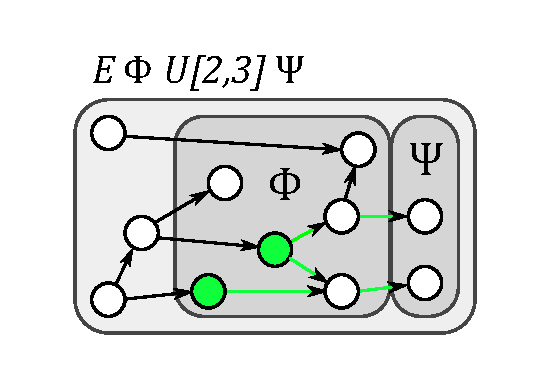
\includegraphics[width=\textwidth]{picture/Graphen/eu_zb.eps}
    \label{fig:eu_zb}
    }
  \end{minipage}
  \caption[Zustandsgraph mit Ergebnismenge einer $E \: \Phi \: U \: \Psi $ - Operation]{Beispielhafter Zustandsgraph f�r die  $E \: \Phi \: U \: \Psi $ - Operation mit Fallunterscheidung in Zeitunbeschr�nkung \ref{fig:eu_zub} und Zeitbeschr�nkung \ref{fig:eu_zb} }
  \label{fig:eu_z}
\end{figure}


...

 \newpage
 

%\chapter{Berechnung des Skalierungsfaktors \label{ch_aus_skal}}
%
%Anhang 2



%%%
%%%
%%%    WOHL EHER NICHT MEHR GEBRAUCHT
%%%
%%%
%\tiny tiny\\
%\scriptsize scriptsize\\
%\footnotesize footnotesize\\
%\small small\\
%\normalsize normalsize\\

%$EF \ \Phi \ \ $ und $ \ \ EF \left[ t_{low}, t_{high} \right] \ \Phi $:
%\small{
%\begin{itemize}
%	\item Existiert mindestens ein Weg, auf dem irgendwann $\Phi$ erf�llt ist? %Zu pr�fende Frage: 
%	\item F�r jeden Zustand in der Ergebnismenge gilt, dass sie die Menge $\Phi$ irgendwann erreichen.
%	\item Teilmengenrelation: $ EF \left[ t_{low}, t_{high} \right] \ \Phi \subseteq EF \ \Phi $ 
%	\item �quivalenzen: 
%   \begin{align}
%	  EF \ \Phi & \equiv \ E \ \textbf{true} \ U \ \Phi \notag \\
%	  EF \left[ t_{low}, t_{high} \right] \ \Phi  \ & \equiv \ E  \ \textbf{true} \ U \left[ 0, t_{high} \right] \ \Phi \notag
%   \end{align}
%\end{itemize}
%}
%\vspace{10mm}
 
\end{appendix}

 \newpage

\end{document}
